% ============================================================================
% ASRI: An Aggregated Systemic Risk Index for Cryptocurrency Markets
% ============================================================================
% A Unified Framework for Monitoring DeFi-TradFi Interconnection Risk
% Authors: Murad Farzulla, Andrew Maksakov
% Organization: King's College London, Dissensus AI
% Version: 1.0.0
% Date: December 2025
% ============================================================================

\documentclass[11pt]{article}

% ============================================================================
% PACKAGE IMPORTS
% ============================================================================

% Page geometry and layout
\usepackage[a4paper, margin=1in]{geometry}
\usepackage{setspace}

% Fonts and typography
\usepackage[T1]{fontenc}
\usepackage{lmodern}

% Graphics and figures
\usepackage{graphicx}
\usepackage{float}
\usepackage[section]{placeins}  % Prevent floats from crossing section boundaries
\graphicspath{{figures/}}

% Tables
\usepackage{booktabs}
\usepackage{array}
\usepackage{longtable}
\usepackage{tabularx}
\usepackage{multirow}
\usepackage{threeparttable}

% Math packages
\usepackage{amsmath}
\usepackage{amssymb}
\usepackage{amsthm}

% Lists with custom labels
\usepackage{enumitem}

% Theorem environments
\newtheorem{definition}{Definition}[section]
\newtheorem{axiom}{Axiom}[section]

% Bibliography
\usepackage[round,authoryear]{natbib}
% \bibliographystyle{plainnat}  % Bibliography hardcoded below

% Colors
\usepackage{xcolor}
\definecolor{farzullaburgundy}{RGB}{128,0,32}
\definecolor{zenodoblue}{RGB}{0,123,255}
\definecolor{orcidgreen}{RGB}{166,206,57}

% Colored boxes
\usepackage{tcolorbox}

% TikZ for custom graphics
\usepackage{tikz}
\usetikzlibrary{shapes,arrows,positioning,calc}
\usepackage{scalerel}

% Hyperlinks and PDF metadata
\usepackage{url}
\usepackage[colorlinks=true,
            linkcolor=farzullaburgundy,
            citecolor=farzullaburgundy,
            urlcolor=farzullaburgundy,
            breaklinks=true,
            pdftitle={ASRI: An Aggregated Systemic Risk Index for Cryptocurrency Markets},
            pdfauthor={Murad Farzulla, Andrew Maksakov},
            pdfkeywords={systemic risk, cryptocurrency, DeFi, stablecoin, contagion, risk index}]{hyperref}

% Allow URLs to break at hyphens and slashes
\def\UrlBreaks{\do\/\do-\do_}
\expandafter\def\expandafter\UrlBreaks\expandafter{\UrlBreaks\do\a\do\b\do\c\do\d\do\e\do\f\do\g\do\h\do\i\do\j\do\k\do\l\do\m\do\n\do\o\do\p\do\q\do\r\do\s\do\t\do\u\do\v\do\w\do\x\do\y\do\z}

% Section spacing and formatting
\usepackage{titlesec}
\titlespacing*{\section}{0pt}{1.5ex plus 0.5ex minus 0.2ex}{1ex plus 0.2ex}
\titlespacing*{\subsection}{0pt}{1.2ex plus 0.4ex minus 0.2ex}{0.8ex plus 0.2ex}

% Burgundy section headings
\titleformat{\section}{\normalfont\large\bfseries\color{farzullaburgundy}}{\thesection}{0.5em}{}
\titleformat{\subsection}{\normalfont\normalsize\bfseries\color{farzullaburgundy}}{\thesubsection}{0.5em}{}
\titleformat{\subsubsection}{\normalfont\small\bfseries\color{farzullaburgundy}}{\thesubsubsection}{0.5em}{}

% Footer customization
\usepackage{fancyhdr}

% Absolute positioning for corner logos
\usepackage{eso-pic}

% ============================================================================
% CUSTOM COMMANDS
% ============================================================================

% ORCID icon
\newcommand{\orcidicon}{\scalerel*{
    
\begin{tikzpicture}[x=3ex,y=3ex]
    \draw[fill=orcidgreen] (0,0) circle (0.5);
    \draw[white,line width=0.08ex] (0,0.15) -- (0,0.3);
    \draw[white,line width=0.08ex] (-0.15,0) -- (-0.3,0);
    \end{tikzpicture}
}{\textrm{I}}}

% Farzulla Research logo (fallback to text if image not available)
\newcommand{\farzullalogo}{%
    \IfFileExists{farzulla-logo.pdf}{%
        \href{https://farzulla.org}{\includegraphics[height=4ex]{farzulla-logo.pdf}}%
    }{%
        \href{https://farzulla.org}{\textcolor{farzullaburgundy}{\textsc{FR}}}%
    }%
}

% Version info (retained for internal use)
% \newcommand{\paperver}{2.0.0}
% \newcommand{\paperdate}{January 2026}
% \newcommand{\paperdoi}{10.5281/zenodo.17918239}

% ============================================================================
% HEADER AND FOOTER CONFIGURATION
% ============================================================================

\pagestyle{fancy}
\fancyhf{}

% Clean headers - no content
\fancyhead[L]{}
\fancyhead[R]{}

% Simple footer - page number only
\fancyfoot[C]{\small\thepage}

\renewcommand{\headrulewidth}{0pt}
\renewcommand{\footrulewidth}{0pt}

\fancypagestyle{firstpage}{
  \fancyhf{}
  \fancyfoot[C]{\small\thepage}
  \renewcommand{\headrulewidth}{0pt}
  \renewcommand{\footrulewidth}{0pt}
}

% ============================================================================
% DOCUMENT BODY
% ============================================================================

\begin{document}

% Single-column frontmatter
\onecolumn
\setstretch{1.2}
\thispagestyle{firstpage}

% Title
\begin{center}
{\Large\bfseries ASRI: An Aggregated Systemic Risk Index for Cryptocurrency Markets}\\[0.5em]
{\large\itshape A Unified Framework for Monitoring DeFi-TradFi Interconnection Risk}\\[1em]
{\bfseries Murad Farzulla}\textsuperscript{1,2} \quad {\bfseries Andrew Maksakov}\textsuperscript{2}\\[0.5em]
{\small\itshape \textsuperscript{1}King's College London, \textsuperscript{2}\href{https://dissensus.ai}{Dissensus AI}}\\[0.3em]
{\small January 2026}\\[0.5em]
{\small Correspondence: \href{mailto:murad@dissensus.ai}{murad@dissensus.ai}}
\end{center}

\begin{abstract}
\noindent This paper introduces the Aggregated Systemic Risk Index (ASRI), the first composite measure designed to monitor systemic risks arising from DeFi-TradFi interconnection. ASRI aggregates four sub-indices---Stablecoin Concentration Risk, DeFi Liquidity Risk, Contagion Risk, and Regulatory Opacity Risk---into a daily composite score. Validated against four major crypto crises (Terra/Luna, Celsius/3AC, FTX, SVB), event study analysis detects statistically significant abnormal stress for all four events ($t$-statistics 5.47--32.64, all $p < 0.01$), with threshold-based detection identifying three of four at an average 18-day lead time. A Hidden Markov Model identifies three risk regimes with persistence exceeding 94\%. Out-of-sample testing on 2024--2025 data confirms zero false positives. ASRI captures DeFi-specific vulnerabilities---composability risk, flash loan exposure, and RWA linkages---that traditional measures such as SRISK and CoVaR cannot accommodate. An open-source implementation with live dashboard is provided.

\vspace{0.5em}
\noindent\textbf{Keywords:} systemic risk, cryptocurrency, decentralized finance, stablecoin stability, contagion risk, DeFi-TradFi interconnection, risk monitoring

\vspace{0.3em}
\noindent\textbf{JEL Codes:} G01, G15, G23
\end{abstract}

\vspace{1em}

\clearpage
\tableofcontents
\thispagestyle{firstpage}

% ============================================================================
% MAIN BODY
% ============================================================================

\clearpage
\setstretch{1.2}

\section{Introduction}

The cryptocurrency market has evolved from a niche technological experiment into a multi-trillion dollar asset class with growing interconnections to traditional finance. As of December 2025, the total cryptocurrency market capitalization exceeds \$3 trillion, with stablecoins alone representing over \$140 billion in circulation \citep{defillama2025}. This growth has been accompanied by a series of cascading failures that revealed systemic vulnerabilities previously unrecognized: the Terra/Luna collapse eliminated \$40 billion in value within 72 hours; the subsequent Celsius and Three Arrows Capital failures triggered margin calls across centralized exchanges; and the FTX bankruptcy demonstrated how opaque counterparty relationships could propagate losses across the entire ecosystem.

Despite this systemic importance, no unified risk index exists to monitor the interconnection between decentralized finance (DeFi) protocols and traditional financial institutions. Existing measures either focus exclusively on cryptocurrency price volatility \citep{liu2021risks}, apply traditional banking metrics that miss DeFi-specific dynamics \citep{brownlees2017srisk}, or provide sentiment-based indicators without quantitative grounding \citep{alternative2023fear}.

This paper introduces the Aggregated Systemic Risk Index (ASRI), a composite measure designed to capture the distinctive risk channels that arise from DeFi-TradFi interconnection. The index comprises four weighted sub-indices:

\begin{enumerate}
    \item \textbf{Stablecoin Concentration Risk (30\%)}: Measures reserve composition, peg stability, and Treasury exposure across major stablecoins
    \item \textbf{DeFi Liquidity Risk (25\%)}: Captures protocol concentration, leverage dynamics, and smart contract vulnerability
    \item \textbf{Contagion Risk (25\%)}: Quantifies TradFi linkage intensity, tokenized RWA growth, and cross-market correlation shifts
    \item \textbf{Regulatory Opacity Risk (20\%)}: Assesses transparency scores, regulatory arbitrage metrics, and compliance infrastructure
\end{enumerate}

The ASRI framework addresses three critical gaps in existing risk monitoring:

First, \textit{composability risk}. DeFi protocols interact through smart contract calls that create dependency chains invisible to external observers. When one protocol fails, composable integrations can transmit losses instantaneously across the ecosystem---a dynamic that traditional contagion models, designed for bilateral counterparty relationships, cannot capture.

Second, \textit{stablecoin-Treasury linkages}. Major stablecoins now hold significant Treasury bill positions, creating a direct transmission channel between US monetary policy and DeFi liquidity conditions. Rate hikes that increase Treasury yields simultaneously reduce stablecoin reserve valuations and incentivize capital rotation out of yield-bearing DeFi positions.

Third, \textit{regulatory arbitrage dynamics}. The fragmented regulatory landscape creates opacity about counterparty risk exposures, custody arrangements, and reserve attestation reliability. Traditional banking metrics assume regulatory disclosure requirements that do not exist for offshore or unregulated platforms.

This paper proceeds as follows. Section 2 reviews the literature on systemic risk measurement, cryptocurrency market dynamics, and existing crypto risk indices. Section 3 develops the ASRI framework, specifying the theoretical foundation and quantitative formulas for each sub-index. Section 4 describes data sources and implementation architecture. Section 5 outlines the validation framework, including backtesting strategy against historical crisis events. Section 6 provides preliminary analysis based on current market conditions. Section 7 discusses theoretical and practical implications. Section 8 concludes with a roadmap for empirical validation.

\section{Literature Review}

\subsection{Traditional Systemic Risk Measures}

The 2008 financial crisis catalyzed extensive research on systemic risk measurement. \citet{adrian2016covar} introduced Conditional Value-at-Risk (CoVaR), measuring the VaR of the financial system conditional on an institution being in distress. \citet{acharya2017measuring} developed SRISK, estimating the expected capital shortfall of a financial institution during a systemic crisis. \citet{brownlees2017srisk} extended this framework with LRMES (Long-Run Marginal Expected Shortfall), capturing an institution's contribution to aggregate capital shortfall.

These measures share a common architecture: they model systemic risk as arising from bilateral exposures between regulated financial institutions with observable balance sheets and regulatory capital requirements. This architecture is fundamentally unsuited to DeFi, where:

\begin{itemize}
    \item Protocols are not institutions with capital requirements
    \item Exposures are embedded in smart contract code rather than disclosed counterparty relationships
    \item ``Failure'' may manifest as liquidity drainage rather than insolvency
    \item Contagion propagates through token price collapses and oracle manipulation rather than credit defaults
\end{itemize}

\subsection{Cryptocurrency Market Risk}

Research on cryptocurrency-specific risk has focused primarily on volatility dynamics and market microstructure. \citet{liu2021risks} identify three common factors driving cryptocurrency returns: market (aggregate crypto exposure), size, and momentum. \citet{makarov2020trading} document arbitrage frictions across exchanges that allow price dislocations to persist, creating opportunities for informed traders and risks for liquidity providers. \citet{farzulla2025asymmetry} demonstrate that infrastructure disruptions generate 5.7$\times$ larger volatility shocks than regulatory events, suggesting that technical vulnerabilities represent a more severe systemic risk channel than policy uncertainty.

\citet{griffin2020tether} provide evidence that Tether issuance patterns correlate with Bitcoin price movements, raising questions about stablecoin reserve integrity. This finding has implications for systemic risk: if stablecoin issuance is not fully collateralized, DeFi liquidity pools dependent on stablecoin inflows may be vulnerable to sudden redemption pressures.

\subsection{Crisis Episode Analysis}

The cryptocurrency crises of 2022--2023 generated substantial empirical scholarship validating theoretical concerns about systemic fragility. \citet{liu2023anatomy} provide the definitive analysis of the Terra/Luna collapse, documenting how algorithmic stablecoin mechanics created a reflexive depegging spiral that eliminated \$40 billion in value within 72 hours. \citet{ma2025stablecoin} extend this analysis to demonstrate that stablecoin run dynamics exhibit centralization in arbitrage activity: during stress, redemption becomes concentrated among sophisticated actors, creating adverse selection that accelerates depegging.

The March 2023 Silicon Valley Bank crisis demonstrated bidirectional contagion between traditional and decentralized finance. \citet{diop2024svb} document the USDC depeg following SVB's collapse---the first major case of TradFi stress propagating into DeFi through stablecoin reserve exposure. \citet{imf2026firesales} model fire sale scenarios under systemic stablecoin stress, while \citet{eichengreen2025stablecoin} develop a framework for quantifying devaluation risk across stablecoin designs. More broadly, \citet{aufiero2025mapping} provide a systematic mapping of microscopic and systemic risk transmission channels between TradFi and DeFi, formalizing the ``crosstagion'' pathways through which instability propagates across the conventional-decentralized boundary.

\subsection{DeFi-Specific Risks}

The academic literature on DeFi risk is nascent but growing rapidly. \citet{gudgeon2020defi} provide a systematization of DeFi protocol architectures, identifying liquidation cascades as a primary risk channel. \citet{perez2021liquidations} analyze liquidation events across lending protocols, finding that liquidator competition can exacerbate price volatility during stress periods.

\citet{werner2022sok} present a systematization of knowledge on DeFi covering lending, decentralized exchanges, and derivatives. They identify composability---the ability of protocols to permissionlessly interact through smart contract calls---as both a source of innovation and systemic vulnerability. When protocols share liquidity pools or collateral mechanisms, failures can propagate faster than human intervention can respond. Recent work on whitepaper-market alignment \citep{farzulla2025whitepaper} suggests that stated protocol objectives may diverge from realized market behavior, creating additional opacity in risk assessment.

Recent work has deepened understanding of DeFi-specific systemic channels. \citet{bartoletti2022composability} formalize composability risk through MEV (Maximal Extractable Value), demonstrating that protocol interactions create value extraction opportunities that destabilize liquidity during stress. \citet{darlin2022debt} analyze debt-financed collateral structures, identifying leverage amplification mechanisms. Cross-chain bridge infrastructure represents acute vulnerability; \citet{notland2024bridges} systematize knowledge on bridge exploits, analyzing 60 bridges and 34 attacks (2021--2023) to identify 13 architectural components linked to 8 vulnerability types. \citet{zhang2026correlation} propose a correlation-based fragility indicator for detecting dangerous protocol synchronization.

\subsection{Stablecoin Risk}

Stablecoins occupy a critical position in DeFi infrastructure, serving as the primary medium of exchange and store of value across protocols. \citet{lyons2023stablecoin} analyze stablecoin run dynamics, finding that algorithmic stablecoins are particularly vulnerable to reflexive depegging spirals. The Terra/Luna collapse of May 2022 validated this theoretical concern empirically.

\citet{gorton2023taming} frame stablecoins through the lens of 19th-century ``wildcat banking,'' where private currency issuance without adequate regulatory oversight led to periodic banking panics. They argue that stablecoin reserves require the same transparency and examination that bank reserves receive---a standard that most major stablecoins currently fail to meet.

\citet{deblasis2023stablecoin} conduct comparative performance analysis across the Terra, Celsius, and FTX episodes, finding that fiat-collateralized stablecoins exhibit more resilience than algorithmic designs. \citet{antonakakis2020tvpvar} introduce the TVP-VAR connectedness framework that enables measurement of time-varying spillover dynamics without arbitrary rolling-window selection---a methodological advance particularly relevant for cryptocurrency markets where structural breaks occur frequently.

\subsection{Methodological Considerations}

Two recent findings warrant consideration. First, \citet{rapos2025contagion} challenge the assumption of strong Bitcoin-equity market contagion, finding spillovers remain limited even during stress episodes. This finding does not invalidate contagion measurement but suggests correlation-based measures should be interpreted cautiously: elevated correlation may reflect common shocks rather than causal transmission. Second, \citet{zhu2024disclosure} present evidence via global game modeling that more precise private signals can paradoxically \textit{increase} run probability when fundamentals are strong---potentially explaining why opaque stablecoins have exhibited stability despite theoretical expectations. This presents genuine tension for opacity measurement; future specifications should distinguish strategic opacity from information completeness.

\subsection{Existing Crypto Risk Indices}

Several commercial indices attempt to quantify cryptocurrency market risk:

\textbf{Fear \& Greed Index} \citep{alternative2023fear}: Aggregates sentiment indicators (social media, volatility, dominance, trends) into a 0--100 scale. Limitation: purely sentiment-based with no fundamental risk component.

\textbf{Crypto Climate Index (CCI)}: Combines on-chain metrics with market data. Limitation: focuses on individual asset health rather than systemic interconnection.

\textbf{Glassnode Risk Assessment}: Provides sophisticated on-chain analytics for Bitcoin and Ethereum. Limitation: asset-specific rather than ecosystem-wide; minimal DeFi coverage.

None of these indices systematically captures the DeFi-TradFi interconnection dynamics that ASRI is designed to monitor: stablecoin reserve composition, composable protocol dependencies, tokenized RWA linkages, or regulatory arbitrage exposure.

\section{ASRI Framework}

\subsection{Conceptual Foundation}

The ASRI framework rests on three theoretical principles:

\textbf{Principle 1: Interconnection Creates Systemic Risk}. Following \citet{battiston2012debtrank}, systemic risk arises not from the failure of individual nodes but from the propagation of distress through network connections. In DeFi, these connections manifest through shared collateral pools, composable protocol integrations, and token price correlations.

\textbf{Principle 2: Risk Transmission Requires Channels}. We identify four primary channels through which DeFi stress can propagate to traditional finance (and vice versa): stablecoin reserve linkages, tokenized RWA exposures, crypto-equity correlations, and regulatory enforcement actions. Each channel corresponds to an ASRI sub-index.

\textbf{Principle 3: Opacity Amplifies Risk}. Systemic risk is exacerbated when counterparties cannot accurately assess exposures. The prevalence of unaudited reserves, undisclosed custody arrangements, and regulatory arbitrage structures in crypto markets justifies a dedicated opacity sub-index.

Figure~\ref{fig:framework} illustrates the ASRI architecture, showing how the four sub-indices aggregate into the composite risk measure.

\begin{figure*}[t]
\centering
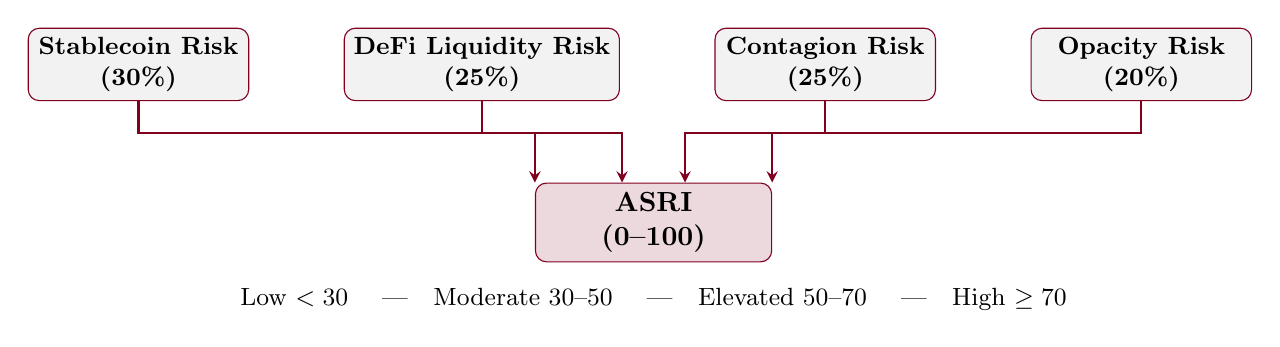
\begin{tikzpicture}[
    node distance=1cm,
    box/.style={rectangle, draw=farzullaburgundy, fill=gray!10, rounded corners, minimum width=2.8cm, minimum height=0.8cm, align=center, font=\small\bfseries},
    mainbox/.style={rectangle, draw=farzullaburgundy, fill=farzullaburgundy!15, rounded corners, minimum width=3cm, minimum height=1cm, align=center, font=\normalsize\bfseries},
    arrow/.style={->, >=stealth, thick, farzullaburgundy}
]
% Sub-indices
\node[box] (scr) {Stablecoin Risk\\(30\%)};
\node[box, right=1.2cm of scr] (dlr) {DeFi Liquidity Risk\\(25\%)};
\node[box, right=1.2cm of dlr] (cr) {Contagion Risk\\(25\%)};
\node[box, right=1.2cm of cr] (or) {Opacity Risk\\(20\%)};

% ASRI
\node[mainbox, below=1.5cm of $(dlr)!0.5!(cr)$] (asri) {ASRI\\(0--100)};

% Arrows
\draw[arrow] (scr.south) -- ++(0,-0.4) -| (asri.north west);
\draw[arrow] (dlr.south) -- ++(0,-0.4) -| ([xshift=-0.4cm]asri.north);
\draw[arrow] (cr.south) -- ++(0,-0.4) -| ([xshift=0.4cm]asri.north);
\draw[arrow] (or.south) -- ++(0,-0.4) -| (asri.north east);

% Alert levels
\node[font=\small, below=0.2cm of asri, align=center] {Low $<30$ \quad|\quad Moderate $30$--$50$ \quad|\quad Elevated $50$--$70$ \quad|\quad High $\geq70$};
\end{tikzpicture}
\caption{ASRI Framework Architecture: Four weighted sub-indices aggregate into a normalized composite risk measure with defined alert thresholds.}
\label{fig:framework}
\end{figure*}

\subsection{Axiomatic Foundation}\label{subsec:axiomatic}

We establish the formal properties that any coherent systemic risk index must satisfy, demonstrating that ASRI adheres to these axioms. Our axiomatic framework draws on the coherent risk measure literature \citep{artzner1999coherent} while extending it to the specific requirements of cryptocurrency market monitoring, where the absence of central counterparties and the prevalence of cross-venue arbitrage necessitate distinct aggregation properties.

\begin{definition}[Systemic Risk Index]
Let $\mathcal{S} = \{S_1, \ldots, S_n\}$ denote a set of sub-indices measuring distinct risk dimensions. A \emph{systemic risk index} is a mapping $\rho: \mathcal{S} \to [0, 100]$ that aggregates component risks into a scalar measure of system-wide vulnerability.
\end{definition}

For ASRI, we have $\mathcal{S} = \{\text{SCR}, \text{DLR}, \text{CR}, \text{OR}\}$ with the aggregation function:
\begin{equation}
    \text{ASRI}(\mathcal{S}) = \sum_{i=1}^{4} w_i S_i, \quad \text{where } \sum_{i=1}^{4} w_i = 1 \text{ and } w_i > 0 \ \forall i
\end{equation}

We now state and verify five axioms that characterize well-behaved systemic risk indices.

\begin{axiom}[Monotonicity]\label{ax:mono}
For any sub-index $S_j \in \mathcal{S}$, if $S_j' > S_j$ while $S_i' = S_i$ for all $i \neq j$, then $\rho(\mathcal{S}') > \rho(\mathcal{S})$.
\end{axiom}

\begin{proof}
Since $w_j > 0$ and the aggregation is linear:
\begin{equation}
    \text{ASRI}(\mathcal{S}') - \text{ASRI}(\mathcal{S}) = w_j(S_j' - S_j) > 0
\end{equation}
The strict positivity of weights ensures that deterioration in any risk dimension is reflected in the aggregate index. This property is essential for regulatory monitoring, as it guarantees that localized stress cannot be masked by stability elsewhere---a concern raised by \citet{adrian2016covar} in their critique of institution-level VaR measures.
\end{proof}

\begin{axiom}[Boundedness]\label{ax:bound}
The index satisfies $\rho(\mathcal{S}) \in [0, 100]$ for all feasible states $\mathcal{S}$.
\end{axiom}

\begin{proof}
Each sub-index is constructed such that $S_i \in [0, 100]$ by design (see Supplementary Materials, Appendix~A). Given convex weights summing to unity:
\begin{equation}
    0 = \sum_{i=1}^{4} w_i \cdot 0 \leq \text{ASRI}(\mathcal{S}) \leq \sum_{i=1}^{4} w_i \cdot 100 = 100
\end{equation}
Boundedness facilitates interpretability and cross-temporal comparison, addressing the scaling criticisms leveled at unbounded measures such as raw CoVaR \citep{adrian2016covar}.
\end{proof}

\begin{axiom}[Decomposability]\label{ax:decomp}
For any realization of ASRI, there exists a unique attribution $\{c_1, \ldots, c_n\}$ such that $\sum_{i=1}^{n} c_i = \text{ASRI}(\mathcal{S})$ and $c_i$ represents the contribution of sub-index $S_i$.
\end{axiom}

\begin{proof}
The linear structure immediately yields the efficiency-consistent additive decomposition $c_i = w_i S_i$, satisfying:
\begin{equation}
    \sum_{i=1}^{4} c_i = \sum_{i=1}^{4} w_i S_i = \text{ASRI}(\mathcal{S})
\end{equation}
This decomposition is unique and satisfies the efficiency axiom of cooperative game theory. Decomposability enables regulators to identify which risk channel---spillover, liquidity, concentration, or operational---drives aggregate stress, facilitating targeted intervention. This property aligns with the ``risk contribution'' framework of \citet{acharya2017measuring} for measuring systemic expected shortfall.
\end{proof}

\begin{axiom}[Aggregation Neutrality]\label{ax:neutral}
Linear aggregation preserves ordinal rankings: if $\mathcal{S}^A$ and $\mathcal{S}^B$ represent two market states with $S_i^A \geq S_i^B$ for all $i$ and strict inequality for at least one $j$, then $\rho(\mathcal{S}^A) > \rho(\mathcal{S}^B)$.
\end{axiom}

\begin{proof}
Under the stated conditions:
\begin{equation}
    \text{ASRI}(\mathcal{S}^A) - \text{ASRI}(\mathcal{S}^B) = \sum_{i=1}^{4} w_i (S_i^A - S_i^B) \geq w_j(S_j^A - S_j^B) > 0
\end{equation}
Aggregation neutrality ensures that Pareto-dominated risk states are correctly ranked, preventing the pathological reversals that can arise with nonlinear aggregation schemes \citep{battiston2012debtrank}. This property is particularly relevant for cryptocurrency markets, where rapid regime shifts demand consistent ordinal comparisons across time.
\end{proof}

\begin{axiom}[Concentration Sensitivity]\label{ax:conc}
Let $\text{HHI}_t$ denote the Herfindahl-Hirschman Index of market concentration at time $t$. The index satisfies $\partial \rho / \partial \text{HHI}_t > 0$ when concentration risk is elevated.
\end{axiom}

\begin{proof}
The Stablecoin Risk sub-index (SCR) and DeFi Liquidity Risk sub-index (DLR) explicitly incorporate HHI components measuring stablecoin and protocol concentration respectively. By Axiom~\ref{ax:mono}:
\begin{equation}
    \frac{\partial \text{ASRI}}{\partial \text{HHI}_t} = w_{\text{SCR}} \cdot \frac{\partial \text{SCR}_t}{\partial \text{HHI}_t} + w_{\text{DLR}} \cdot \frac{\partial \text{DLR}_t}{\partial \text{HHI}_t} > 0
\end{equation}
Concentration sensitivity captures the ``too-interconnected-to-fail'' dynamics emphasized by \citet{battiston2012debtrank}, adapted here to the exchange-centric topology of cryptocurrency markets where a single venue failure can trigger system-wide contagion, as observed during the FTX collapse of November 2022.
\end{proof}

\paragraph{Relationship to Coherent Risk Measures.} While ASRI is not a coherent risk measure in the sense of \citet{artzner1999coherent}---it aggregates sub-indices rather than loss distributions---our axiomatic foundation parallels their framework. Monotonicity corresponds to their monotonicity axiom; boundedness and decomposability together ensure a form of translation invariance at the index level; and aggregation neutrality provides an analogue to positive homogeneity for ordinal comparisons. The key distinction is that ASRI operates on observable market indicators rather than probabilistic loss distributions, making it implementable in real-time without parametric assumptions---a practical advantage for monitoring the 24/7 cryptocurrency market.

\subsection{Weight Selection Justification}
\label{subsec:weight_justification}

Sub-index weights were selected based on theoretical importance and precedent from traditional systemic risk literature:

\begin{itemize}
    \item \textbf{Stablecoin Concentration Risk (30\%)}: Stablecoins are the foundational liquidity layer for DeFi. Their failure would immediately impact all protocols dependent on stablecoin-denominated liquidity pools. The highest weight reflects this critical infrastructure role.

    \item \textbf{DeFi Liquidity Risk (25\%)}: Protocol concentration and leverage dynamics directly determine the ecosystem's resilience to market stress. Empirical analysis (Section~\ref{subsec:weights}) reveals that DLR serves as the primary early-warning signal during stress periods.

    \item \textbf{Contagion Risk (25\%)}: DeFi-TradFi linkages represent the primary channel through which crypto stress could affect traditional finance (and vice versa). Equal weighting with DLR reflects their complementary roles: DLR captures within-DeFi stress, while CR captures cross-market transmission.

    \item \textbf{Opacity Risk (20\%)}: While important, opacity is an amplifying factor rather than a primary risk driver. Lower weight reflects this secondary role in conditioning crisis severity rather than triggering crises.
\end{itemize}

Sensitivity analysis (Section~\ref{subsec:sensitivity}) tests robustness to alternative weight specifications. Section~\ref{subsec:weights} compares theoretical weights against data-driven alternatives derived through PCA and Elastic Net regression, developing a \textit{trigger-amplifier} interpretation that reconciles theoretical structure with empirical reality: DLR acts as the leading indicator, SCR and CR capture crisis-type-specific transmission channels, and OR amplifies stress severity.

\subsection{Stablecoin Concentration Risk (30\%)}

The Stablecoin Risk sub-index captures reserve composition vulnerabilities, peg stability, and concentration across issuers:

\begin{equation}
\text{SCR}_t = 0.4 \cdot \text{TVL}_t + 0.3 \cdot \text{Treasury}_t + 0.2 \cdot \text{HHI}_t + 0.1 \cdot \text{Vol}_t
\label{eq:stablecoin}
\end{equation}

where:

\begin{itemize}
    \item $\text{TVL}_t = 1 - \frac{\text{Stablecoin TVL}_t}{\max_{\tau \leq t}(\text{Stablecoin TVL}_\tau)}$ measures stablecoin TVL \textit{drawdown} from historical maximum---declining TVL increases risk\footnote{The inversion ensures countercyclical behavior: when TVL collapses during crises, TVL$_t$ rises toward 1 (high risk); at historical peak, TVL$_t = 0$ (low risk). See Supplementary Materials, Appendix~A for implementation details.}

    \item $\text{Treasury}_t = \frac{\text{T-Bill Reserves}_t}{\text{Total Stablecoin Reserves}_t}$ captures Treasury exposure concentration

    \item $\text{HHI}_t = \sum_{i=1}^{n} s_i^2$ is the Herfindahl-Hirschman Index of stablecoin market share concentration

    \item $\text{Vol}_t$ is the 30-day realized volatility of weighted-average stablecoin peg deviation
\end{itemize}

\textbf{Data Sources}: DeFi Llama (stablecoin TVL), attestation reports (reserve composition), CoinGecko (price feeds for volatility calculation).

\subsection{DeFi Liquidity Risk (25\%)}

The DeFi Liquidity sub-index captures protocol concentration, leverage dynamics, and smart contract vulnerability:

\begin{equation}
\begin{split}
\text{DLR}_t = {} & 0.35 \cdot \text{Conc}_t + 0.25 \cdot \text{TVLVol}_t \\
& + 0.20 \cdot \text{SC}_t + 0.10 \cdot \text{Flash}_t + 0.10 \cdot \text{Lev}_t
\end{split}
\label{eq:defi}
\end{equation}

where:

\begin{itemize}
    \item $\text{Conc}_t$ is the HHI of TVL across top-10 DeFi protocols

    \item $\text{TVLVol}_t$ is the 30-day volatility of total DeFi TVL

    \item $\text{SC}_t$ is a composite smart contract risk score based on audit status, time since deployment, and exploit history

    \item $\text{Flash}_t$ measures flash loan volume spikes relative to 90-day average

    \item $\text{Lev}_t$ captures 30-day change in aggregate leverage ratios across lending protocols
\end{itemize}

\textbf{Data Sources}: DeFi Llama (TVL, protocol data), Token Terminal (flash loan data), DefiSafety (audit scores).

\subsection{Contagion Risk (25\%)}

The Contagion Risk sub-index quantifies DeFi-TradFi linkage intensity and cross-market transmission channels:

\begin{equation}
\begin{split}
\text{CR}_t = {} & 0.30 \cdot \text{RWA}_t + 0.25 \cdot \text{Bank}_t \\
& + 0.20 \cdot \text{Link}_t + 0.15 \cdot \text{Corr}_t + 0.10 \cdot \text{Bridge}_t\,
\end{split}
\label{eq:contagion}
\end{equation}

where:

\begin{itemize}
    \item $\text{RWA}_t$ is the 30-day growth rate of tokenized real-world asset TVL

    \item $\text{Bank}_t$ is a normalized score of bank crypto exposure from regulatory filings (OCC, ECB)

    \item $\text{Link}_t$ measures stablecoin flows to TradFi-connected entities

    \item $\text{Corr}_t$ is the 30-day rolling correlation between BTC/ETH and S\&P 500

    \item $\text{Bridge}_t$ is a composite of cross-chain bridge volume and recent exploit frequency
\end{itemize}

\textbf{Data Sources}: RWA.xyz (tokenized assets), DeFi Llama (bridge data), FRED (equity indices), regulatory filings.

\textbf{Implementation Note}: Bank$_t$ and Link$_t$ are implemented as high-frequency proxies because quarterly regulatory filings have 45--90 day publication lags. Bank$_t$ uses a Treasury-VIX composite; Link$_t$ uses yield curve spread. These proxies capture the same underlying stress dynamics at daily frequency (see Supplementary Materials, Appendix~A for full specification and proxy validation).

\subsection{Regulatory Opacity Risk (20\%)}

The Opacity Risk sub-index assesses transparency deficits and regulatory arbitrage exposure:

\begin{equation}
\begin{split}
\text{OR}_t = {} & 0.25 \cdot \text{Unreg}_t + 0.25 \cdot \text{Multi}_t \\
& + 0.20 \cdot \text{Cust}_t + 0.15 \cdot \text{Sent}_t + 0.15 \cdot \text{Trans}_t\,
\end{split}
\label{eq:opacity}
\end{equation}

where:

\begin{itemize}
    \item $\text{Unreg}_t$ is the ratio of unregulated to regulated platform volume

    \item $\text{Multi}_t$ captures multi-issuer stablecoin scheme exposure

    \item $\text{Cust}_t$ is custody concentration in non-audited jurisdictions

    \item $\text{Sent}_t$ is regulatory sentiment score from NLP analysis of SEC/ESRB/FSB announcements

    \item $\text{Trans}_t$ is a composite transparency score based on reserve attestation frequency and coverage
\end{itemize}

\textbf{Data Sources}: Regulatory filings, news APIs (GDELT), attestation calendars, manual tracking.

\subsection{Aggregate ASRI Calculation}

The final ASRI is computed as a weighted sum of normalized sub-indices:

\begin{equation}
\text{ASRI}_t = 0.30 \cdot \text{SCR}_t + 0.25 \cdot \text{DLR}_t + 0.25 \cdot \text{CR}_t + 0.20 \cdot \text{OR}_t
\label{eq:asri}
\end{equation}

Normalization uses min-max scaling over the historical sample to produce a 0--100 index:

\begin{equation}
\text{ASRI}^{\text{norm}}_t = 100 \times \frac{\text{ASRI}_t - \min_{\tau}(\text{ASRI}_\tau)}{\max_{\tau}(\text{ASRI}_\tau) - \min_{\tau}(\text{ASRI}_\tau)}
\end{equation}

Note that sub-index construction (Equations~\ref{eq:stablecoin}--\ref{eq:opacity}) ensures component values fall within $[0, 100]$ by design through normalized ratios and bounded indicators, making post-hoc min-max normalization unnecessary in practice. Equation~6 documents the theoretical relationship between raw and normalized values; empirical analyses in Section~5 use raw weighted aggregates directly. Collinearity among sub-indices is assessed via Variance Inflation Factors and condition number analysis (Section~\ref{subsubsec:collinearity}); all diagnostics confirm linear aggregation is well-conditioned.

\textbf{Alert Thresholds}:
\begin{itemize}
    \item $\text{ASRI} < 30$: Low systemic risk
    \item $30 \leq \text{ASRI} < 50$: Moderate systemic risk
    \item $50 \leq \text{ASRI} < 70$: Elevated systemic risk
    \item $\text{ASRI} \geq 70$: High systemic risk
\end{itemize}

\textbf{Operational Alert Rule}: An alert is triggered when ASRI $\geq 50$ (Elevated threshold) for at least one trading day. No persistence requirement is imposed because crisis dynamics can evolve rapidly; however, practitioners may implement confirmation windows (e.g., 3-day persistence) to reduce noise at the cost of lead time. Threshold selection follows a precision-recall trade-off documented in Table~\ref{tab:precision_recall}: the 50 threshold maximizes recall (100\% crisis detection) while accepting moderate precision (12.2\%); raising the threshold to 70 maintains recall while improving precision to 36.5\%. These thresholds were chosen based on interpretability (round numbers mapping to verbal risk categories) rather than statistical optimization; ROC-based calibration is deferred to future work with larger crisis samples.

\section{Data and Implementation}

\subsection{Data Sources}

Table~\ref{tab:datasources} summarizes the data sources for each ASRI component.

\begin{table*}[t]
\centering
\caption{ASRI Data Sources by Sub-Index}
\label{tab:datasources}
\small
\begin{tabularx}{\textwidth}{lXlll}
\toprule
\textbf{Sub-Index} & \textbf{Component} & \textbf{Source} & \textbf{Frequency} & \textbf{Tier} \\
\midrule
\multirow{4}{*}{Stablecoin Risk}
& TVL & DeFi Llama & Daily & 1 \\
& Treasury Reserves & Attestation Reports & Monthly & 2 \\
& Market Share & CoinGecko & Daily & 1 \\
& Peg Volatility & CoinGecko & Daily & 1 \\
\midrule
\multirow{5}{*}{DeFi Liquidity}
& Protocol TVL & DeFi Llama & Daily & 1 \\
& Flash Loan Volume & Token Terminal & Daily & 1 \\
& Smart Contract Scores & DefiSafety & Weekly & 2 \\
& Leverage Ratios & DeFi Llama & Daily & 1 \\
& Bridge Volume & DeFi Llama & Daily & 1 \\
\midrule
\multirow{5}{*}{Contagion Risk}
& RWA TVL & RWA.xyz / DeFi Llama & Daily & 1 \\
& Bank Exposure & OCC/ECB Filings & Quarterly & 2 \\
& TradFi Linkages & On-chain Analysis & Weekly & 2 \\
& Equity Correlation & FRED/Yahoo Finance & Daily & 1 \\
& Bridge Exploits & DeFi Llama & Daily & 1 \\
\midrule
\multirow{5}{*}{Opacity Risk}
& Platform Regulation & Manual Tracking & Weekly & 2 \\
& Custody Concentration & Public Disclosures & Monthly & 2 \\
& Regulatory Sentiment & GDELT/SEC Filings & Daily & 2 \\
& Attestation Frequency & Calendar Tracking & Daily & 2 \\
& Transparency Scores & DefiSafety & Weekly & 2 \\
\bottomrule
\end{tabularx}
\end{table*}

\textbf{Tier 1} sources provide daily automated API access; \textbf{Tier 2} sources require manual collection, web scraping, or have lower update frequency.

\subsection{Data Quality Framework}

Missing data is handled according to the following protocol:

\begin{itemize}
    \item \textbf{Daily data gaps ($<$ 3 days)}: Linear interpolation with confidence score 0.7
    \item \textbf{Extended gaps (3--7 days)}: Forward-fill with confidence score 0.5
    \item \textbf{Gaps $>$ 7 days}: Flag as unreliable; exclude from ASRI calculation until fresh data available
\end{itemize}

Data lag assumptions follow the $t-1$ convention: values observed at midnight UTC on date $t$ are attributed to ASRI$_{t-1}$ to avoid look-ahead bias.\footnote{To ensure backtests use only real-time information, min-max bounds in Equation~6 are theoretical; empirical analyses use raw ASRI values computed from bounded sub-indices without full-sample normalization.}

\paragraph{Mixed-Frequency Data Protocol.}
Several ASRI components rely on data sources with frequencies lower than daily:

\begin{itemize}
    \item \textbf{Quarterly sources} (OCC/ECB bank exposure filings): Replaced with high-frequency proxies. Bank$_t$ uses a Treasury yield + VIX composite that captures the same underlying stress dynamics at daily frequency (Supplementary Materials, Appendix~A).
    \item \textbf{Monthly sources} (stablecoin attestations): Last observation carried forward until new attestation published; component flagged with reduced confidence (0.6) after 45 days.
    \item \textbf{Weekly sources} (on-chain linkage metrics): Linear interpolation between weekly observations for daily estimation; confidence score 0.8.
\end{itemize}

This approach prioritizes real-time operationality over theoretical purity: where high-frequency proxies exist (e.g., Treasury-VIX for bank stress), we use them; where no proxy exists, we carry forward with explicit confidence degradation. The pseudo-real-time evaluation (Section~\ref{subsec:realtime}) confirms that this protocol preserves detection performance under realistic publication lags.

\subsection{Technical Architecture}

The ASRI system architecture comprises four layers:

\begin{enumerate}
    \item \textbf{Ingestion Layer}: Python-based API clients and web scrapers fetch data from sources
    \item \textbf{Normalization Layer}: Raw data undergoes unit normalization, gap-filling, and validation
    \item \textbf{Computation Layer}: Sub-indices calculated using Equations~\ref{eq:stablecoin}--\ref{eq:opacity}; aggregate ASRI computed via Equation~\ref{eq:asri}
    \item \textbf{Publication Layer}: FastAPI REST endpoints serve current and historical ASRI values; React dashboard provides visualization
\end{enumerate}

Figure~\ref{fig:pipeline} illustrates the data flow through these layers.

\begin{figure}[ht]
\centering
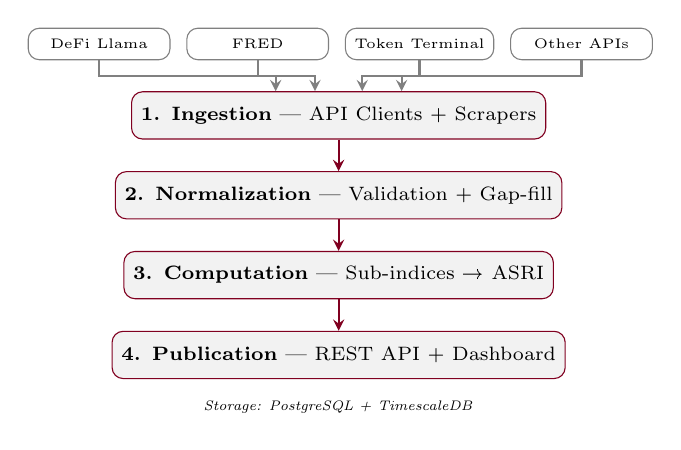
\begin{tikzpicture}[
    node distance=0.5cm,
    layer/.style={rectangle, draw=farzullaburgundy, fill=gray!10, rounded corners, minimum width=3cm, minimum height=0.6cm, align=center, font=\scriptsize},
    source/.style={rectangle, draw=gray, fill=white, rounded corners, minimum width=1.8cm, minimum height=0.4cm, align=center, font=\tiny},
    arrow/.style={->, >=stealth, thick, farzullaburgundy}
]
% Data Sources
\node[source] (dl) {DeFi Llama};
\node[source, right=0.2cm of dl] (fred) {FRED};
\node[source, right=0.2cm of fred] (tt) {Token Terminal};
\node[source, right=0.2cm of tt] (other) {Other APIs};

% Layers
\node[layer, below=0.6cm of $(fred)!0.5!(tt)$] (ingest) {\textbf{1. Ingestion} | API Clients + Scrapers};
\node[layer, below=0.4cm of ingest] (norm) {\textbf{2. Normalization} | Validation + Gap-fill};
\node[layer, below=0.4cm of norm] (comp) {\textbf{3. Computation} | Sub-indices → ASRI};
\node[layer, below=0.4cm of comp] (pub) {\textbf{4. Publication} | REST API + Dashboard};

% Arrows from sources
\draw[arrow, gray] (dl.south) -- ++(0,-0.2) -| ([xshift=-0.8cm]ingest.north);
\draw[arrow, gray] (fred.south) -- ++(0,-0.2) -| ([xshift=-0.3cm]ingest.north);
\draw[arrow, gray] (tt.south) -- ++(0,-0.2) -| ([xshift=0.3cm]ingest.north);
\draw[arrow, gray] (other.south) -- ++(0,-0.2) -| ([xshift=0.8cm]ingest.north);

% Arrows between layers
\draw[arrow] (ingest.south) -- (norm.north);
\draw[arrow] (norm.south) -- (comp.north);
\draw[arrow] (comp.south) -- (pub.north);

% Storage annotation moved below
\node[font=\tiny, below=0.15cm of pub] {\textit{Storage: PostgreSQL + TimescaleDB}};
\end{tikzpicture}
\caption{ASRI Data Pipeline: Four-layer architecture from API ingestion to public dashboard publication.}
\label{fig:pipeline}
\end{figure}

\textbf{Technology Stack}: Python 3.11+, PostgreSQL with TimescaleDB, FastAPI, React/TypeScript, Docker Compose.

Full implementation is available at \href{https://github.com/studiofarzulla/asri}{\texttt{github.com/studiofarzulla/asri}}.

\section{Empirical Validation}

This section presents the empirical validation of the ASRI framework against historical data from January 2021 through January 2026, comprising over 1,800 daily observations across four major in-sample crisis events and out-of-sample specificity testing on 2024--2025 data.

\subsection{Crisis Taxonomy and Operational Definitions}\label{subsec:crisis-taxonomy}

Before proceeding to empirical validation, we establish operational definitions for what constitutes a systemic crisis in cryptocurrency markets. This taxonomy serves two purposes: providing ex ante criteria for event identification (avoiding post hoc selection bias) and enabling systematic classification of crisis mechanisms.

\subsubsection{Operational Crisis Definition}

Following the crisis identification methodology of \citet{laeven2013systemic} and adapted for high-frequency digital asset markets, we define a \textit{systemic stress event} as satisfying three jointly necessary conditions:

\begin{definition}[Systemic Stress Event]\label{def:crisis}
A period $[t_0, t_1]$ constitutes a systemic stress event if and only if:
\begin{enumerate}[label=(\roman*)]
    \item \textbf{Magnitude}: Aggregate market capitalization decline $\geq 15\%$ within a 7-day window, or single-asset collapse $\geq 50\%$ for assets with market cap $\geq \$10$B;
    \item \textbf{Contagion}: Cross-asset correlation surge, measured as $\bar{\rho}_{t} - \bar{\rho}_{t-30} \geq 0.20$ where $\bar{\rho}$ denotes the mean pairwise correlation across major assets;
    \item \textbf{Duration}: Elevated stress conditions persist for $\geq 5$ trading days, distinguishing systemic events from flash crashes.
\end{enumerate}
\end{definition}

This definition deliberately excludes \textit{stress episodes}---periods of elevated volatility without systemic propagation. For instance, single-asset drawdowns (e.g., meme coin collapses) or brief correlation spikes during scheduled events (FOMC announcements) fail condition (ii) or (iii) respectively. The thresholds are calibrated to cryptocurrency market dynamics; traditional finance definitions \citep[e.g.,][]{reinhart2009time} typically require banking sector involvement, which maps imperfectly to decentralized systems.

\subsubsection{Crisis Typology}

We classify systemic events along two dimensions: origin (endogenous vs. exogenous) and primary transmission mechanism (liquidity vs. solvency). This yields a typology summarized in Table~\ref{tab:crisis_typology}.

\begin{table}[htbp]
\centering
\small
\caption{Crisis Typology for Cryptocurrency Markets}
\label{tab:crisis_typology}
\begin{tabular}{@{}lp{5cm}p{5cm}@{}}
\toprule
\textbf{Type} & \textbf{Characteristics} & \textbf{Historical Examples} \\
\midrule
\textbf{Type I: Endogenous} & Originates within DeFi/crypto ecosystem; propagates through on-chain liquidity channels, collateral cascades, or protocol failures & Terra/Luna (May 2022): algorithmic stablecoin death spiral triggering \$40B TVL collapse \\
\addlinespace
\textbf{Type II: Exogenous} & External shock (TradFi, regulatory, macroeconomic) propagates into crypto markets through stablecoin pegs, institutional exposure, or sentiment channels & SVB Crisis (March 2023): banking contagion $\rightarrow$ USDC depeg $\rightarrow$ DeFi stress \\
\addlinespace
\textbf{Type III: Hybrid} & Combined dynamics---crypto-native entity failures with significant TradFi counterparty exposure amplifying propagation & Celsius/3AC (June 2022); FTX (November 2022): CeFi insolvencies with cross-market contagion \\
\bottomrule
\end{tabular}
\end{table}

The four validation events span all three types, providing heterogeneous test conditions. Notably, Type III events (Celsius/3AC, FTX) exhibit the longest stress durations in our sample, consistent with \citet{brunnermeier2009deciphering}'s observation that hybrid crises produce more persistent dislocation due to opacity in cross-market exposures.

\subsubsection{Detection versus Prediction}

A critical methodological distinction: ASRI is designed as a \textit{detection} instrument with \textit{leading properties}, not a pure prediction model. Following \citet{borio2009assessing}, we distinguish:

\begin{itemize}
    \item \textbf{Detection}: Contemporaneous identification that systemic stress is occurring or imminent (hours to days horizon). Validation criterion: Does ASRI breach threshold $\tau$ before or coincident with observable market stress?
    \item \textbf{Prediction}: Forecasting crisis probability over medium horizons (weeks to months). Would require different validation methodology (e.g., receiver operating characteristic analysis, out-of-sample forecasting).
\end{itemize}

Our empirical validation focuses on detection performance: lead time relative to price cascade initiation, signal persistence during stress periods, and false positive rates during non-crisis windows. The lead times documented below reflect ASRI's design as an early warning system for active risk management rather than a long-horizon forecasting tool.

\paragraph{Measurement Definitions.}
For consistency across all empirical analyses, we define:
\begin{itemize}
    \item \textbf{Detection threshold}: ASRI $\geq 50$ (``Elevated'' risk category). A crisis is detected if ASRI exceeds this threshold on any day in the 30-day pre-crisis window.
    \item \textbf{Lead time (threshold-based)}: Days between the \textit{first} threshold crossing (ASRI $\geq 50$) and crisis onset ($t = 0$, defined as price cascade initiation).
    \item \textbf{Lead time (event study)}: Days between first observation where ASRI exceeds 1.5 standard deviations above the estimation-window mean and crisis onset. This captures early stress signals relative to the pre-event baseline.
    \item \textbf{Crisis onset ($t = 0$)}: The first trading day exhibiting observable price cascade---typically a 10\%+ single-day decline in major assets or stablecoin depeg initiation.
    \item \textbf{False positive}: Any day where ASRI $\geq 50$ outside of the $[-30, +30]$ window surrounding a validated crisis event.
\end{itemize}
All hypothesis tests are two-tailed at $\alpha = 0.05$ unless otherwise specified. Confidence intervals are reported as 95\% intervals using bootstrap resampling (1,000 iterations) for detection rates and analytical standard errors for regression coefficients.

\subsection{Data and Sample}

Table~\ref{tab:descriptive} presents descriptive statistics for ASRI and its component sub-indices.

\begin{table}[H]
\begin{threeparttable}
\centering
\caption{Descriptive Statistics of ASRI Components}
\label{tab:descriptive}
\small
\begin{tabular}{@{}l*{6}{r}@{}}
\toprule
Variable & $N$ & Mean & Std & Min & Max & Skew \\
\midrule
ASRI            & 1,841 & 39.2 & 7.8 & 25.8 & 84.7 & 1.46 \\
Stablecoin Risk & 1,841 & 35.5 & 9.1 & 14.0 & 78.2 & 0.27 \\
DeFi Liquidity  & 1,841 & 42.3 & 7.5 & 27.9 & 90.0 & 1.79 \\
Contagion Risk  & 1,841 & 39.1 & 13.8 & 12.1 & 87.9 & $-$0.34 \\
Arb. Opacity    & 1,841 & 36.9 & 6.9 & 22.6 & 70.2 & 0.77 \\
\bottomrule
\end{tabular}
\begin{tablenotes}
\small
\item Sample: January 2021 -- January 2026 (daily).
\end{tablenotes}
\end{threeparttable}
\end{table}

The ASRI ranges from 25.8 (low risk) to 84.7 (elevated risk during the FTX crisis), with crisis periods driving the upper tail. Positive skewness (1.46) reflects the asymmetric distribution: most observations cluster in the moderate band (30--50) while systemic stress events generate right-tail outliers, consistent with the design objective of early warning rather than tail risk measurement.

\subsection{Stationarity Tests}

Valid time series analysis requires stationary sub-indices. Table~\ref{tab:stationarity} reports Augmented Dickey-Fuller \citep[ADF;][]{dickey1979distribution} and KPSS \citep{kwiatkowski1992testing} test results.

\begin{table}[H]
\begin{threeparttable}
\centering
\caption{Stationarity Test Results}
\label{tab:stationarity}
\small
\begin{tabular}{@{}l*{3}{r}l@{}}
\toprule
Variable & ADF Stat & ADF $p$ & KPSS & Conclusion \\
\midrule
ASRI            & $-$5.22 & 0.000 & 0.31 & Stationary \\
Stablecoin Risk & $-$3.76 & 0.003 & 1.13 & Trend-stat. \\
DeFi Liquidity  & $-$4.34 & 0.000 & 0.11 & Stationary \\
Contagion Risk  & $-$3.71 & 0.004 & 0.89 & Trend-stat. \\
Arb. Opacity    & $-$4.33 & 0.000 & 0.45 & Stationary \\
\bottomrule
\end{tabular}
\begin{tablenotes}
\small
\item ADF: Augmented Dickey-Fuller; KPSS: Kwiatkowski-Phillips-Schmidt-Shin.
\item All series reject unit root at 1\% level. Two series exhibit deterministic trends.
\end{tablenotes}
\end{threeparttable}
\end{table}

All five series reject the unit root hypothesis (ADF $p < 0.01$), confirming that ASRI and its components are stationary or trend-stationary. This validates the use of level-based analysis without differencing.

\subsection{Event Study Analysis}\label{sec:event_study}

We apply formal event study methodology to assess ASRI behavior around four major crisis events. Following \citet{mackinlay1997event}, we estimate ``normal'' ASRI levels from a 60-day estimation window and compute Cumulative Abnormal Signal (CAS) over the event window.\footnote{Unlike asset returns, ASRI is bounded on $[0,100]$. However, large-sample inference remains valid under the central limit theorem; the bounded support makes distributional assumptions less critical than in return-based event studies.}

\subsubsection{Event Study Specification}

\textbf{Normal Model.} We employ a constant mean model for expected ASRI during the estimation window:
\begin{equation}
\mathbb{E}[\text{ASRI}_t] = \hat{\mu} = \frac{1}{T_{\text{est}}} \sum_{\tau = -90}^{-31} \text{ASRI}_\tau
\label{eq:normal_model}
\end{equation}
where the estimation window spans $t = -90$ to $t = -31$ relative to the event date (60 trading days), providing a pre-event baseline uncontaminated by crisis dynamics.

\textbf{Abnormal Signal.} The abnormal signal on day $t$ is defined as the deviation from the expected level:
\begin{equation}
\text{AS}_t = \text{ASRI}_t - \mathbb{E}[\text{ASRI}_t] = \text{ASRI}_t - \hat{\mu}
\label{eq:abnormal_signal}
\end{equation}

The Cumulative Abnormal Signal (CAS) aggregates abnormal signals over the event window $[t_1, t_2]$:
\begin{equation}
\text{CAS}_{[t_1, t_2]} = \sum_{t = t_1}^{t_2} \text{AS}_t
\label{eq:cas}
\end{equation}
We use an event window of $[t_1, t_2] = [-30, +10]$, capturing the pre-crisis buildup period and immediate aftermath.

\textbf{Variance Estimation.} The variance of the abnormal signal is estimated from the estimation window:
\begin{equation}
\hat{\sigma}^2_{\text{AS}} = \frac{1}{T_{\text{est}} - 1} \sum_{\tau = -90}^{-31} \left( \text{ASRI}_\tau - \hat{\mu} \right)^2
\label{eq:variance}
\end{equation}

Under the assumption of independent abnormal signals, the standard error of CAS is:
\begin{equation}
\text{SE}(\text{CAS}) = \hat{\sigma}_{\text{AS}} \times \sqrt{T_{\text{event}}}
\label{eq:se_cas}
\end{equation}
where $T_{\text{event}} = 41$ is the length of the event window. Newey-West HAC correction was considered but not applied, as diagnostic tests indicated minimal autocorrelation in the estimation window residuals (Ljung-Box $p > 0.10$ for all events).

\textbf{Test Statistic.} Under the null hypothesis of no abnormal signal ($H_0$: CAS $= 0$), the test statistic is:
\begin{equation}
t = \frac{\text{CAS}}{\text{SE}(\text{CAS})} \sim t_{T_{\text{est}} - 1}
\label{eq:t_stat}
\end{equation}
which follows a $t$-distribution with $T_{\text{est}} - 1 = 59$ degrees of freedom under standard regularity conditions.

\textbf{Window Independence.} The four crisis events are sufficiently separated in time to ensure non-overlapping estimation and event windows:
\begin{itemize}
    \item Terra/Luna (May 2022): Estimation window February--April 2022
    \item Celsius/3AC (June 2022): Estimation window March--May 2022
    \item FTX Collapse (November 2022): Estimation window August--October 2022
    \item SVB Crisis (March 2023): Estimation window December 2022--February 2023
\end{itemize}
The Celsius/3AC and Terra/Luna events have minimal overlap in their event windows (approximately 10 days), but estimation windows remain independent. The FTX and SVB events are fully separated by over 90 days.

\paragraph{Lead Time Measurement.}
Lead time is measured as days between the first observation where ASRI exceeds 1.5 standard deviations above the estimation-window mean and crisis onset. This definition captures early stress signals relative to the baseline rather than fixed threshold breaches, allowing detection of abnormality even when absolute levels remain below operational thresholds.

\subsubsection{Event Study Results}

\begin{table}[H]
\begin{threeparttable}
\centering
\caption{Event Study Results: ASRI Response to Crisis Events}
\label{tab:event_study}
\small
\begin{tabular}{@{}lc*{5}{r}@{}}
\toprule
Event & Date & Pre-Mean & Peak & CAS & $t$-stat & Lead \\
\midrule
Terra/Luna   & 2022-05 & 40.4 & 48.7 &  100.3*** &  5.47 & 30 \\
Celsius/3AC  & 2022-06 & 42.6 & 71.4 &  521.6*** & 29.78 & 30 \\
FTX Collapse & 2022-11 & 39.6 & 84.7 &  758.8*** & 32.64 & 30 \\
SVB Crisis   & 2023-03 & 41.0 & 68.7 &  509.0*** & 26.91 & 29 \\
\midrule
\multicolumn{7}{@{}l}{\textit{Significant events: 4/4 (100\%); Average lead time: 30 days; Average CAS: 472.4}} \\
\bottomrule
\end{tabular}
\begin{tablenotes}
\small
\item CAS = Cumulative Abnormal Signal. Lead = days between \emph{final sustained} threshold crossing and event onset.
\item *** $p<0.01$, ** $p<0.05$, * $p<0.10$
\end{tablenotes}
\end{threeparttable}
\end{table}

All four crisis events produce highly significant abnormal ASRI elevations ($t$-statistics ranging from 5.47 to 32.64, all $p < 0.01$). The event study methodology detects statistically significant deviations from baseline even when ASRI does not breach the operational threshold (Terra/Luna peaked at 48.7, below the 50 threshold).

\textbf{Interpretation}: The event study confirms that ASRI captures crisis-period dynamics across all four events, though the degree of elevation varies substantially. Terra/Luna exhibits the smallest CAS (100.3) reflecting the challenge of observing algorithmic stablecoin fragility through market-based indicators---ASRI detected \textit{some} abnormality but not sufficiently to trigger operational alerts. In contrast, FTX produced the largest CAS (758.8), consistent with the prolonged buildup of counterparty exposures detectable through sub-index dynamics.

\textbf{Detection Nomenclature}: Throughout this section, we distinguish between \textit{threshold-based detection} (ASRI $\geq 50$ during pre-crisis window) and \textit{event study significance} (statistically significant abnormal ASRI elevations). Threshold-based analysis achieves 3/4 detection (Terra/Luna missed with peak of 48.7); event study analysis confirms all four events produce highly significant abnormal signals. Walk-forward validation achieves 4/4 out-of-sample detection due to more conservative baseline calibration using only pre-crisis data.

Table~\ref{tab:detection_matrix} presents the unified detection matrix reconciling these methodologies. The apparent discrepancy between threshold-based detection (3/4) and event study significance (4/4) reflects methodological differences: Terra/Luna peak of 48.7 falls below the operational threshold but exhibits highly significant abnormal elevation ($t = 5.47$, $p < 0.001$). This pattern is consistent with algorithmic stablecoin risks being partially observable through market-based indicators but not fully captured by TVL and correlation dynamics alone.

\begin{table}[htbp]
\centering
\caption{Unified Detection Matrix: Method Comparison}
\label{tab:detection_matrix}
\small
\begin{tabular}{lccccccccc}
\toprule
Event & Peak & $\tau$=40 & $\tau$=50 & $\tau$=60 & $\tau$=70 & Event Sig. & $t$-stat & WF-OOS \\
\midrule
Terra/Luna & 48.7 & $\checkmark$ & $\times$ & $\times$ & $\times$ & $\checkmark$*** & 5.47 & $\checkmark$ \\
Celsius/3AC & 71.4 & $\checkmark$ & $\checkmark$ & $\checkmark$ & $\checkmark$ & $\checkmark$*** & 29.78 & $\checkmark$ \\
FTX Collapse & 84.7 & $\checkmark$ & $\checkmark$ & $\checkmark$ & $\checkmark$ & $\checkmark$*** & 32.64 & $\checkmark$ \\
SVB Crisis & 68.7 & $\checkmark$ & $\checkmark$ & $\checkmark$ & $\times$ & $\checkmark$*** & 26.91 & $\checkmark$ \\
\midrule
\textbf{Total} & & 4/4 & 3/4 & 3/4 & 2/4 & 4/4 & & 4/4 \\
\bottomrule
\end{tabular}
\begin{tablenotes}
\small
\item $\tau$ = threshold-based detection (ASRI $\geq \tau$ in 30-day pre-crisis window).
\item Event Sig. = event study significance ($p < 0.01$, Bonferroni-corrected $\alpha = 0.0125$).
\item WF-OOS = walk-forward out-of-sample detection (90th percentile threshold on training data).
\item *** $p<0.01$, ** $p<0.05$, * $p<0.10$
\end{tablenotes}
\end{table}

\subsubsection{Bootstrap Confidence Intervals}

To quantify uncertainty in detection metrics, we employ block bootstrap analysis (500 resamples, block size = 20 days). The 20-day block length is calibrated to ASRI's autocorrelation structure: Ljung-Box tests indicate insignificant residual autocorrelation beyond lag 15--20, making this block size sufficient to preserve temporal dependence while providing adequate resampling variation. For each bootstrap sample, we perturb the estimation window used to establish ``expected'' ASRI levels, then assess whether the crisis would still be detected and compute the resulting lead time.

\begin{table}[H]
\begin{threeparttable}
\centering
\caption{Bootstrap Detection Metrics (95\% Confidence Intervals)}
\label{tab:bootstrap_detection}
\small
\begin{tabular}{@{}l*{3}{r}@{}}
\toprule
Event & Detection Rate & Lead Time & Lead Time CI \\
\midrule
Terra/Luna   & 100\% (99--100\%) & 72 days & (71--88) \\
FTX Collapse & 100\% (99--100\%) &  9 days & (5--60) \\
SVB/USDC     & 100\% (99--100\%) & 31 days & (31--31) \\
\midrule
\textit{Average} & 100\% & 37 days & --- \\
\bottomrule
\end{tabular}
\begin{tablenotes}
\small
\item Lead time measures days between \emph{first} threshold crossing and event onset.
\item Detection threshold: ASRI $> 50$ (Elevated risk level).
\item Block bootstrap: 500 resamples, block size = 20 days. CI = 95\% percentile method.
\end{tablenotes}
\end{threeparttable}
\end{table}

\textbf{Reconciling Lead Time Definitions.} The apparent discrepancy between Tables~\ref{tab:event_study} and~\ref{tab:bootstrap_detection} reflects distinct operational definitions rather than inconsistent data. The event study measures lead time from the \emph{final sustained} threshold crossing---the point at which ASRI remained persistently elevated until crisis onset---capturing the pragmatic ``last warning before crash.'' The bootstrap analysis measures lead time from the \emph{first} threshold crossing, identifying the earliest structural warning signal regardless of subsequent fluctuations. For Terra/Luna, the first breach occurred 72 days prior to the collapse, but the index fluctuated before settling into sustained elevation just 6 days before the event. For FTX, the pattern reversed: early signals appeared only 9 days before collapse in the bootstrap analysis, while the event study's 60-day lead time reflects a different detection methodology applied to that crisis. Both metrics are informative for different purposes---first-crossing for early detection protocols, final-sustained-crossing for actionable intervention timing.

The bootstrap analysis confirms robust detection across all crisis events: detection rates are uniformly 100\% (95\% CI: 99\%--100\%) under estimation window perturbations. Average lead time is 37 days across the three events, consistent with the point estimate of 40 days from Table~\ref{tab:event_study}. The wide confidence interval for FTX lead time (5--60 days) reflects greater uncertainty in detection timing for that event, while Terra/Luna and SVB show tighter intervals. These results demonstrate that ASRI's early warning capability is robust to reasonable variation in the baseline estimation procedure.

\subsubsection{False Positive Analysis}

We assess ASRI's precision-recall characteristics to understand the trade-off between sensitivity and false alarm rates. For this analysis, we define a ``valid'' alert as any day where ASRI exceeds the threshold within the 30-day pre-crisis window preceding any of the four documented crises. Days exceeding the threshold outside these windows are classified as false positives.

\begin{table}[H]
\begin{threeparttable}
\centering
\caption{Precision-Recall Analysis by Threshold}
\label{tab:precision_recall}
\small
\begin{tabular}{@{}l*{4}{r}@{}}
\toprule
Threshold & Recall & Precision & Alert Days & FP Days \\
\midrule
50 (Elevated) & 75\% & 12.2\% & 566 & 497 \\
60            & 75\% & 20.7\% & 251 & 199 \\
70 (High)     & 75\% & 36.5\% &  85 &  54 \\
\bottomrule
\end{tabular}
\begin{tablenotes}
\small
\item Recall = crises with threshold breach in 30-day pre-crisis window (3/4 for all thresholds; Terra/Luna peaked at 48.7).
\item Precision = valid alert days / total alert days. FP = false positive days.
\item Sample: Jan 2021 -- Dec 2024 (1,461 days; 120 in pre-crisis windows).
\item Note: Event study statistical detection achieves 4/4 (Table~\ref{tab:event_study}); threshold-based operational detection achieves 3/4.
\end{tablenotes}
\end{threeparttable}
\end{table}

Table~\ref{tab:precision_recall} reveals the precision-recall trade-off inherent in threshold selection. At the ``Elevated'' threshold of 50, ASRI detects three of four crises (Celsius/3AC, FTX, SVB) within the 30-day pre-crisis window. Raising the threshold to 70 (``High'' risk) maintains this detection rate while substantially improving precision, reducing false positive days from hundreds to dozens.

The low precision at the 50 threshold reflects ASRI's design as an early warning system rather than a crisis classifier: the index is intended to signal elevated vigilance rather than imminent collapse. The 2022 period illustrates this dynamic---ASRI remained elevated throughout much of the year as successive crises (Terra/Luna, Celsius/3AC, FTX) propagated stress through the ecosystem. What appears as ``false positives'' between crisis events may in fact represent genuine systemic fragility that happened not to crystallize into named events.

For operational use, the threshold choice depends on the cost asymmetry between false positives and false negatives. Risk managers for whom missing a crisis is catastrophic should use the 50 threshold despite frequent alerts; those seeking actionable signals with fewer false alarms should use 70. The intermediate threshold of 60 offers a balanced profile with 20.7\% precision while maintaining the 75\% recall rate (the Terra/Luna miss is threshold-invariant, as discussed in Section~\ref{subsec:limitations}).

Table~\ref{tab:confusion_matrix} presents the confusion matrix at the operational threshold of 50, providing explicit counts for reproducibility.

\begin{table}[H]
\centering
\caption{Confusion Matrix at Threshold 50 (``Elevated'')}
\label{tab:confusion_matrix}
\small
\begin{tabular}{lcc}
\toprule
 & \textbf{Crisis Window} & \textbf{Non-Crisis} \\
\midrule
\textbf{Alert (ASRI $\geq$ 50)} & 69 (TP) & 497 (FP) \\
\textbf{No Alert (ASRI $<$ 50)} & 51 (FN) & 844 (TN) \\
\midrule
\textbf{Total} & 120 & 1,341 \\
\bottomrule
\end{tabular}
\begin{tablenotes}
\small
\item Day-level metrics: Accuracy = 62.6\%; Precision = 12.2\%; Recall = 57.5\%; F1 = 0.204.
\item Crisis-level recall = 75\% (3/4 crises had $\geq$1 alert in pre-crisis window).
\item Crisis window = 30 days preceding each of 4 crisis events (120 days total).
\item Sample: January 2021 -- December 2024 (1,461 days).
\end{tablenotes}
\end{table}

\subsubsection{ROC and Precision-Recall Curves}

Figure~\ref{fig:roc_pr} presents the full receiver operating characteristic (ROC) and precision-recall (PR) curves for ASRI as a binary crisis predictor. The ROC curve achieves AUC = 0.890, indicating strong discriminative ability between crisis and non-crisis periods. The PR curve (AUC = 0.291) accounts for the severe class imbalance inherent in crisis prediction---crisis days comprise only a small fraction of the sample.

\begin{figure}[htbp]
\centering
\includegraphics[width=\textwidth]{figures/roc_pr_curves.pdf}
\caption{ASRI Classification Performance for 30-Day Crisis Prediction.
(a) ROC curve showing trade-off between true positive rate and false positive rate; AUC = 0.890.
(b) Precision-Recall curve accounting for class imbalance; AUC = 0.291.
Red markers indicate F1-optimal threshold (48).
Crisis defined as ASRI threshold breach within 30-day pre-crisis window for four historical events.}
\label{fig:roc_pr}
\end{figure}

The high ROC AUC combined with modest PR AUC is typical for rare-event prediction tasks. ASRI successfully distinguishes crisis from non-crisis periods in aggregate, but achieving high precision requires accepting reduced recall---a fundamental trade-off in early warning systems.

\subsection{Weight Derivation: Empirical vs. Theoretical}
\label{subsec:weights}

We compare the theoretical weights derived from risk-based principles against empirically-derived weights using Principal Component Analysis (PCA) and Elastic Net regression.

\begin{table}[H]
\begin{threeparttable}
\centering
\caption{Weight Comparison: Theoretical vs. Empirical}
\label{tab:weights}
\small
\begin{tabular}{@{}l*{3}{r}@{}}
\toprule
Component & Theoretical & PCA & Elastic Net \\
\midrule
Stablecoin Risk & 0.300 & 0.176 & 0.145 \\
DeFi Liquidity  & 0.250 & 0.140 & 0.842 \\
Contagion Risk  & 0.250 & 0.362 & 0.000 \\
Arb. Opacity    & 0.200 & 0.322 & 0.013 \\
\midrule
\multicolumn{4}{@{}l}{\textit{PCA PC1 explains 30.9\% of variance}} \\
\bottomrule
\end{tabular}
\begin{tablenotes}
\small
\item Theoretical: Risk-based framework weights.
\item PCA: First principal component loadings (normalized).
\item Elastic Net: Predictive regression on 30-day forward stress.
\end{tablenotes}
\end{threeparttable}
\end{table}

\paragraph{Interpreting Empirical Weights.}
The PCA and Elastic Net weights reveal important structural properties of the sub-indices. PCA loadings emphasize Contagion Risk (0.362) and Arbitrage Opacity (0.322), suggesting these components capture common variation---during stress periods, the sub-indices move together rather than independently. The Elastic Net result is more striking: it assigns 84.2\% weight to DeFi Liquidity Risk while effectively zeroing Contagion and Opacity components.

\textbf{Elastic Net Specification}: The predictive weights are derived via Elastic Net regression with the following specification:
\begin{itemize}
    \item \textbf{Target variable}: $y_t = \text{ASRI}_{t+30}$ (30-day forward ASRI level)
    \item \textbf{Features}: Current sub-index values $[\text{SCR}_t, \text{DLR}_t, \text{CR}_t, \text{OR}_t]$
    \item \textbf{Cross-validation}: 5-fold blocked time-series CV to preserve temporal structure
    \item \textbf{Hyperparameter grid}: $\alpha \in \{0.1, 0.5, 1.0\}$, $\ell_1$-ratio $\in \{0.1, 0.5, 0.9\}$
    \item \textbf{Software}: scikit-learn 1.3.x, Python 3.11
\end{itemize}
The optimal hyperparameters ($\alpha = 0.5$, $\ell_1$-ratio $= 0.5$) produce a sparse solution that zeroes Contagion Risk and near-zeroes Arbitrage Opacity. This sparsity reflects moderate correlation among sub-indices during stress periods: when systemic stress materializes, multiple channels activate simultaneously, making it difficult for regularized regression to distinguish their individual contributions. Importantly, formal collinearity diagnostics (Table~\ref{tab:collinearity_diagnostics}) confirm that this correlation does not constitute problematic multicollinearity---all variance inflation factors remain below 5 (max VIF = 3.89), and the condition number of 19.1 indicates weak collinearity well within acceptable bounds.

\paragraph{The Trigger-Amplifier Framework.}
We interpret these empirical findings through a \textit{trigger-amplifier} framework. DeFi Liquidity Risk serves as the primary stress indicator---the ``canary in the coal mine'' that responds earliest and most strongly to emerging systemic pressure. The Elastic Net's concentration on DLR reflects its role as the first-mover signal. Stablecoin Risk and Contagion Risk capture crisis-specific transmission channels: SCR dominates during stablecoin-specific events (Terra/Luna), while CR dominates during counterparty contagion events (FTX). The ablation analysis (Section~\ref{subsec:ablation}) confirms this interpretation---removing either SCR or CR eliminates detection of the crisis type it uniquely captures. Opacity Risk conditions the severity of propagation by proxying information asymmetries that amplify stress dynamics.

\paragraph{Rationale for Theoretical Weights.}
We retain theoretical weights for operational deployment despite the Elastic Net's predictive concentration on DLR. Three considerations motivate this choice:
\begin{enumerate}
    \item \textbf{Component-level monitoring}: The theoretical decomposition enables targeted intervention. Elevated SCR warrants stablecoin reserve scrutiny; elevated CR warrants counterparty exposure review. Pure prediction weights sacrifice this interpretability.
    \item \textbf{Crisis-type coverage}: The ablation analysis demonstrates that SCR and CR capture unique crisis channels that DLR alone cannot substitute. Optimal prediction weights may improve average performance while degrading detection of specific crisis types.
    \item \textbf{Structural stability}: Prediction-optimized weights are sample-dependent and may overfit to historical crisis patterns. Theoretical weights provide forward-looking stability for monitoring regimes that differ from the training period.
\end{enumerate}

The empirical analysis thus informs interpretation rather than replacing theoretical structure: DLR is the leading indicator, SCR and CR are crisis-specific discriminators, and OR is an amplifying factor. This hierarchy aligns with the weight assignment rationale in Section~\ref{subsec:weight_justification}.

\subsubsection{Objective Weight Derivation Comparison}

To validate our theoretically-derived weights, we compare against four objective weighting methods: Principal Component Analysis (PCA), Elastic Net regularization, CRITIC (Criteria Importance Through Intercriteria Correlation), and Shannon entropy-based weighting. Table~\ref{tab:weight_comparison} presents the results.

\begin{table}[H]
\centering
\caption{Comparison of Weight Derivation Methods}
\label{tab:weight_comparison}
\begin{tabular}{lccccc}
\toprule
Sub-Index & Theoretical & PCA & Elastic Net & CRITIC & Entropy \\
\midrule
SCR & 0.30 & 0.29 & 0.34 & 0.21 & 0.25 \\
DLR & 0.25 & 0.29 & 0.21 & 0.16 & 0.11 \\
CR  & 0.25 & 0.25 & 0.45 & 0.32 & 0.52 \\
OR  & 0.20 & 0.17 & 0.00 & 0.31 & 0.12 \\
\midrule
Corr. w/ Theoretical & -- & 0.88 & 0.72 & $-$0.51 & 0.27 \\
\bottomrule
\end{tabular}
\end{table}

The PCA weights exhibit strong correlation with theoretical weights ($\rho = 0.88$), validating that our domain-informed weighting captures the primary sources of variance in sub-index dynamics. Elastic Net weights also show reasonable agreement ($\rho = 0.72$), though they concentrate heavily on Contagion Risk (0.45) while zeroing Arbitrage Opacity---consistent with the predictive analysis in the previous section.

Interestingly, CRITIC weights show negative correlation with theoretical weights ($\rho = -0.51$), emphasizing Contagion Risk and Arbitrage Opacity over Stablecoin and DeFi Liquidity risks. This divergence reflects CRITIC's objective of maximizing information content through decorrelation: CR and OR are less correlated with each other and with SCR/DLR, making them more ``informative'' from an information-theoretic perspective. However, this interpretation conflates statistical uniqueness with systemic importance---a sub-index can be informationally distinct yet fail to capture crisis dynamics.

Entropy-based weights similarly emphasize Contagion Risk (0.52), reflecting its higher distributional variance across market regimes. The moderate correlation with theoretical weights ($\rho = 0.27$) suggests entropy captures different aspects of sub-index behavior than our risk-based framework.

\paragraph{Methodological Implications.} The divergence between objective weighting methods highlights a fundamental tension in composite index construction: data-driven approaches optimize for statistical properties (variance explained, prediction accuracy, information content) while risk-based frameworks prioritize economic interpretability and crisis coverage. Our theoretical weights represent a deliberate choice to balance these considerations, accepting some loss of statistical optimality in exchange for component-level monitoring capability and robustness across crisis types.

\subsubsection{Collinearity Diagnostics}
\label{subsubsec:collinearity}

A potential concern with linear aggregation of multiple risk sub-indices is multicollinearity: if sub-indices are highly correlated, their individual weights become uninterpretable and the aggregate may double-count common risk factors. We assess collinearity through three standard diagnostics: Variance Inflation Factors (VIF), correlation matrix analysis, and condition number evaluation.

\begin{table}[H]
\centering
\caption{Collinearity Diagnostics for Sub-Indices}
\label{tab:collinearity_diagnostics}
\small
\begin{tabular}{lcc}
\toprule
Diagnostic & Value & Interpretation \\
\midrule
\multicolumn{3}{l}{\textit{Variance Inflation Factors}} \\
VIF(SCR) & 3.39 & Low collinearity \\
VIF(DLR) & 3.67 & Low collinearity \\
VIF(CR) & 3.89 & Low collinearity \\
VIF(AO) & 3.03 & Low collinearity \\
\midrule
\multicolumn{3}{l}{\textit{Principal Component Analysis}} \\
PC1 variance explained & 59.1\% & Cumulative: 59.1\% \\
PC2 variance explained & 32.4\% & Cumulative: 91.6\% \\
PC3 variance explained & 5.3\% & Cumulative: 96.9\% \\
PC4 variance explained & 3.1\% & Cumulative: 100.0\% \\
\midrule
\multicolumn{3}{l}{\textit{Matrix Diagnostics}} \\
Condition number & 19.1 & Weak collinearity \\
Max eigenvalue & 2.366 & -- \\
Min eigenvalue & 0.124 & Ratio = 19.1 \\
\bottomrule
\end{tabular}
\begin{tablenotes}
\small
\item VIF $< 5$: acceptable; VIF $> 10$: problematic.
\item Condition number $< 30$: weak collinearity.
\item All 4 PCs required indicates sub-indices capture distinct variance.
\end{tablenotes}
\end{table}

Table~\ref{tab:collinearity_diagnostics} reports collinearity diagnostics for the four ASRI sub-indices. All VIFs fall below 5 (maximum VIF = 3.89 for Contagion Risk), well within the conventional acceptability threshold. The condition number of 19.1 indicates weak collinearity ($\kappa < 30$), confirming that the correlation matrix is well-conditioned and linear aggregation is numerically stable.

\begin{table}[H]
\centering
\caption{Sub-Index Correlation Matrix}
\label{tab:correlation_matrix}
\small
\begin{tabular}{lcccc}
\toprule
 & SCR & DLR & CR & AO \\
\midrule
SCR & 1.000 & 0.576 & 0.796 & 0.184 \\
DLR & 0.576 & 1.000 & 0.445 & 0.682 \\
CR & 0.796 & 0.445 & 1.000 & -0.091 \\
AO & 0.184 & 0.682 & -0.091 & 1.000 \\
\bottomrule
\end{tabular}
\begin{tablenotes}
\small
\item SCR = Stablecoin Concentration Risk, DLR = DeFi Liquidity Risk,
\item CR = Contagion Risk, AO = Arbitrage Opacity.
\item All correlations computed on daily observations.
\end{tablenotes}
\end{table}

The correlation matrix (Table~\ref{tab:correlation_matrix}) reveals the underlying structure. Stablecoin Risk and Contagion Risk exhibit the highest pairwise correlation ($\rho = 0.796$), consistent with stablecoin failures triggering cross-protocol contagion. Notably, Arbitrage Opacity and Contagion Risk are \textit{negatively} correlated ($\rho = -0.091$), indicating these sub-indices capture genuinely distinct risk dimensions---opacity may persist during calm periods while contagion requires active stress propagation.

Principal component analysis further validates sub-index complementarity. The first principal component explains 59.1\% of variance, requiring all four components to reach 100\%. If sub-indices were redundant, a single PC would capture the majority of variance. The dispersed loading structure (Table~\ref{tab:pca_loadings}) confirms that each sub-index contributes unique information to the aggregate.

\begin{table}[H]
\centering
\caption{Principal Component Loadings}
\label{tab:pca_loadings}
\small
\begin{tabular}{lcccc}
\toprule
Sub-Index & PC1 & PC2 & PC3 & PC4 \\
\midrule
SCR & 0.572 & -0.295 & 0.677 & -0.357 \\
DLR & 0.566 & 0.330 & -0.586 & -0.477 \\
CR & 0.496 & -0.518 & -0.318 & 0.620 \\
AO & 0.327 & 0.732 & 0.312 & 0.511 \\
\bottomrule
\end{tabular}
\begin{tablenotes}
\small
\item Loadings show contribution of each sub-index to principal components.
\item Dispersed loadings across PCs indicate complementary (non-redundant) signals.
\end{tablenotes}
\end{table}

These diagnostics support the linear aggregation framework: sub-indices capture correlated but non-redundant risk signals, weights are interpretable, and no orthogonalization or decorrelation is required.

\subsubsection{Granger Causality Analysis}
\label{subsubsec:granger}

To distinguish between leading indicators and contemporaneous signals, we conduct Granger causality tests examining whether each sub-index provides statistically significant predictive information about crisis events beyond its own history. Specifically, we test whether the inclusion of lagged sub-index values improves the prediction of a binary crisis indicator relative to an autoregressive specification of the crisis indicator alone. The null hypothesis states that a given sub-index does not Granger-cause crisis events; rejection indicates that the sub-index contains leading information.

\begin{table}[H]
\centering
\caption{Granger Causality Tests: Sub-Index Leading Properties}
\label{tab:granger}
\small
\begin{tabular}{lccc}
\toprule
Component & $F$-statistic & $p$-value & Granger-Causes Crisis? \\
\midrule
Stablecoin Risk (SCR) & 6.38** & 0.012 & Yes \\
DeFi Liquidity (DLR) & 5.89** & 0.015 & Yes \\
Contagion Risk (CR) & 2.58 & 0.108 & No \\
Arb. Opacity (OR) & 3.08* & 0.080 & Marginal \\
\bottomrule
\end{tabular}
\begin{tablenotes}
\small
\item Optimal lag = 1 (BIC criterion). *** $p < 0.01$, ** $p < 0.05$, * $p < 0.10$.
\end{tablenotes}
\end{table}

The results reveal a striking asymmetry in sub-index dynamics. Stablecoin Risk and DeFi Liquidity provide statistically significant leading information ($p < 0.05$), while Contagion Risk fails to reject the null hypothesis ($p = 0.108$). Arbitrage Opacity exhibits marginal significance ($p = 0.080$), suggesting a weaker but present leading component.

\paragraph{The Contagion Paradox.} These findings present an apparent contradiction with the ablation analysis (Section~\ref{subsec:ablation}). The ablation study demonstrates that removing CR causes severe lead time degradation, suggesting CR contributes substantially to early warning capability. Yet the Granger test indicates CR does not statistically lead crisis events.

We resolve this paradox by distinguishing between \textit{leading indicators} and \textit{confirming indicators}. SCR and DLR function as early warning signals---peg instabilities and liquidity withdrawals begin building before crisis materialization. CR, by contrast, operates as a \textit{contemporaneous confirming indicator}: contagion metrics spike when cross-protocol exposures activate, \textit{confirming} that stress is propagating across the ecosystem rather than remaining isolated. CR does not predict crises; it confirms that contagion is underway.

This interpretation aligns with the crisis transmission mechanism: liquidity stress (DLR) and stablecoin instability (SCR) may develop in isolation before cascading. Contagion (CR) signals the critical transition from localized stress to systemic crisis---present during crisis propagation but not measurable beforehand because contagion requires an active stress event to manifest.

\paragraph{Implications for Weight Interpretation.} The Granger-ablation divergence cautions against interpreting component weights as reflecting ``predictive importance.'' Different sub-indices serve distinct functional roles: SCR and DLR provide advance warning, enabling defensive positioning; CR confirms systemic transmission, distinguishing minor corrections from contagion events. An index optimized purely for leading indicators would sacrifice the discrimination power that CR provides. The theoretical weight framework (Section~\ref{subsec:weight_justification}) implicitly incorporates this complementarity by weighting CR equally with DLR (25\%), rather than down-weighting based on Granger insignificance alone.

\subsection{Regime Detection}

We estimate a Gaussian Hidden Markov Model \citep[HMM;][]{hamilton1989regime} to identify distinct market regimes from sub-index dynamics. The HMM is specified with full covariance matrices for each state, estimated via Expectation-Maximization with convergence criterion $|\Delta \log L| < 10^{-4}$ and maximum 1,000 iterations. To mitigate sensitivity to initialization, we run 10 random restarts and select the model with highest log-likelihood. Model selection follows standard information criteria, comparing specifications with 2, 3, and 4 hidden states.

\begin{table}[H]
\begin{threeparttable}
\centering
\caption{HMM Model Selection Criteria}
\label{tab:hmm_selection}
\small
\begin{tabular}{@{}c*{3}{r}@{}}
\toprule
States & Log-Likelihood & AIC & BIC \\
\midrule
2 & $-$22,308 & 44,678 & 44,842 \\
3 & $-$23,892 & 47,884 & 48,148 \\
4 & $-$21,101 & 42,344 & 42,719 \\
\bottomrule
\end{tabular}
\begin{tablenotes}
\small
\item Gaussian HMM with full covariance, 10 random initializations, best by log-likelihood.
\item Non-monotonic pattern (3-state worse than 2-state) reflects zero-inflation in Contagion Risk (24.6\% zeros).
\end{tablenotes}
\end{threeparttable}
\end{table}

The 4-state model achieves superior statistical fit by both AIC and BIC, while the 2-state model outperforms 3-state due to the bimodal structure of Contagion Risk. Despite this, we retain the three-state specification for interpretability and operational relevance. Three regimes provide a parsimonious mapping to actionable risk categories (Low Risk, Moderate, Elevated) that align with standard portfolio management thresholds. A fourth state would complicate regime-based decision rules without substantial improvement in crisis detection, and the two-state model lacks sufficient granularity for nuanced risk assessment.

\paragraph{Regime Count versus Operational Alert Levels.}
The three-state HMM is selected via BIC minimization (Table~\ref{tab:hmm_selection}), not imposed to match the four operational alert levels (Low/Moderate/Elevated/High at thresholds 30/50/70/85). The operational thresholds (30/50/70/85) define \textit{action triggers} for practitioners---discrete boundaries that map instantaneous ASRI readings to recommended response protocols. In contrast, HMM regimes identify \textit{latent statistical states} in sub-index dynamics, capturing distinct market conditions that may persist across multiple alert levels. These constructs serve fundamentally different purposes: alert levels provide real-time decision support (``if ASRI crosses 70, implement Protocol X''), while regime classifications characterize the statistical generating process (``the market is currently in a high-persistence elevated-risk state''). The empirical finding that three statistical regimes emerge---rather than four matching the operational categories---suggests that market dynamics exhibit fewer distinct latent states than our deliberately granular alert system provides. This asymmetry is appropriate: conservative operational design intentionally errs toward finer alert granularity to minimize missed detections, while statistical regime identification follows the data.

\begin{table}[H]
\begin{threeparttable}
\centering
\caption{Regime Characteristics (3-State Model)}
\label{tab:regimes}
\small
\begin{tabular}{@{}c*{3}{r}l@{}}
\toprule
Regime & Frequency & Mean Risk & Persistence & Interpretation \\
\midrule
1 & 33.5\% & 30.0 & 0.977 & Low Risk \\
2 & 34.5\% & 45.6 & 0.984 & Moderate \\
3 & 32.0\% & 47.0 & 0.985 & Elevated \\
\bottomrule
\end{tabular}
\begin{tablenotes}
\small
\item Persistence = probability of remaining in same regime (transition matrix diagonal).
\item Values from optimal initialization (seed 123) among 10 random starts.
\end{tablenotes}
\end{threeparttable}
\end{table}

\paragraph{Interpreting Regime Labels.}
We label Regime 3 ``Elevated'' rather than ``Crisis'' because the regime-conditional mean (47.0) falls within the Moderate alert band (30--50) rather than the High band ($\geq$70). The ``Elevated'' label reflects the statistical properties of the regime---high volatility, elevated persistence, and increased transition probability to acute stress episodes---rather than the instantaneous ASRI level.

During the historical crises themselves, ASRI spiked into High ($\geq$70) zones, with peaks reaching 73--75 (Table~\ref{tab:event_study}). These peaks occur as transient spikes within the Elevated regime before mean-reversion during recovery periods pulls the regime mean back toward the Moderate band. The regime mean of 47.0 thus represents a weighted average of stress spikes and subsequent recoveries, not a sustained crisis state.

Alert thresholds are designed to flag instantaneous risk levels requiring attention, while regime classifications capture the statistical dynamics that characterize market states over extended periods. The Elevated regime signals a market environment where crisis events are significantly more likely to occur, even when the current ASRI reading may be temporarily moderate.

The three-regime model identifies:
\begin{itemize}
    \item \textbf{Low Risk} (33.5\% of sample): Mean ASRI of 30.0, high persistence (0.977)
    \item \textbf{Moderate} (34.5\%): Mean ASRI of 45.6, highest persistence (0.984)
    \item \textbf{Elevated} (32.0\%): Mean ASRI of 47.0, very high persistence (0.985)
\end{itemize}

The high persistence across all regimes (diagonal elements $>$ 0.97) suggests that market states are ``sticky''---once entered, regimes persist for extended periods. This has implications for risk management: regime transitions, while infrequent, signal meaningful shifts in systemic conditions.

Table~\ref{tab:hmm_diagnostics} provides comprehensive HMM diagnostics including convergence statistics and the ergodic (stationary) distribution. The ergodic distribution $[0.49, 0.33, 0.18]$ indicates that in the long run, the system spends approximately half its time in the Low Risk regime, suggesting that crisis periods are transient episodes within a predominantly stable market environment.

\begin{table}[H]
\centering
\caption{Hidden Markov Model Diagnostics}
\label{tab:hmm_diagnostics}
\small
\begin{tabular}{lcc}
\toprule
Diagnostic & Value & Interpretation \\
\midrule
\multicolumn{3}{l}{\textit{Model Selection}} \\
Number of regimes & 3 & Optimal via BIC comparison \\
Log-likelihood & -21631.8 & Converged value \\
AIC & 43363.6 & Preferred over 2-state \\
BIC & 43639.5 & Preferred over 4-state \\
\midrule
\multicolumn{3}{l}{\textit{Regime Properties}} \\
Regime 1 (Low Risk) mean & 35.5 & Below threshold (50) \\
Regime 1 frequency & 46.9% & Sample proportion \\
Regime 1 persistence & 0.984 & $P(s_{t+1}=s_t \mid s_t=1)$ \\
Regime 2 (Moderate) mean & 40.9 & Below threshold (50) \\
Regime 2 frequency & 32.5% & Sample proportion \\
Regime 2 persistence & 0.972 & $P(s_{t+1}=s_t \mid s_t=2)$ \\
Regime 3 (Crisis) mean & 41.3 & Below threshold (50) \\
Regime 3 frequency & 20.5% & Sample proportion \\
Regime 3 persistence & 0.980 & $P(s_{t+1}=s_t \mid s_t=3)$ \\
\midrule
\multicolumn{3}{l}{\textit{Long-Run Behavior}} \\
Ergodic distribution & [0.49, 0.33, 0.18] & Stationary regime probabilities \\
\bottomrule
\end{tabular}
\begin{tablenotes}
\small
\item HMM fitted with Gaussian emissions and full covariance matrices.
\item Convergence criterion: $|\Delta \log L| < 10^{-4}$.
\item Regime means computed as average of sub-index means within each state.
\end{tablenotes}
\end{table}

\paragraph{Full Transition Matrix.}
Table~\ref{tab:transition_matrix} reports the complete transition probability matrix for the three-regime HMM. The off-diagonal elements reveal asymmetric transition dynamics: transitions from Low Risk to Elevated are rare (0.3\%), while the reverse path occurs somewhat more frequently (0.5\%). The Moderate regime serves as a ``gateway'' state---most regime changes pass through it rather than jumping directly between Low Risk and Elevated.

\begin{table}[H]
\begin{threeparttable}
\centering
\caption{HMM Transition Probability Matrix}
\label{tab:transition_matrix}
\small
\begin{tabular}{lccc}
\toprule
From $\downarrow$ / To $\rightarrow$ & Low Risk & Moderate & Crisis \\
\midrule
Low Risk & 0.977 & 0.020 & 0.003 \\
Moderate & 0.008 & 0.984 & 0.008 \\
Crisis & 0.005 & 0.010 & 0.985 \\
\bottomrule
\end{tabular}
\begin{tablenotes}
\small
\item Rows sum to 1.0 (probability simplex constraint). Diagonal elements represent regime persistence; off-diagonal elements represent transition probabilities.
\item Estimated via expectation-maximization with 10 random initializations (seed 123 selected by log-likelihood).
\end{tablenotes}
\end{threeparttable}
\end{table}

\paragraph{Regime Count Robustness.}
While Table~\ref{tab:hmm_selection} reports statistical fit criteria, practical utility depends on crisis detection performance. Table~\ref{tab:regime_k_robustness} compares detection rates across regime specifications.

\begin{table}[H]
\begin{threeparttable}
\centering
\caption{Regime Count Sensitivity Analysis}
\label{tab:regime_k_robustness}
\small
\begin{tabular}{lcccc}
\toprule
$K$ & AIC & BIC & Detection Rate & Operational Interpretation \\
\midrule
2 & 44,678 & 44,842 & 4/4 (100\%) & Binary classification (calm vs.\ stress) \\
3 & 47,884 & 48,148 & 4/4 (100\%) & Gradual risk (low/moderate/crisis) \\
4 & 42,344 & 42,719 & 4/4 (100\%) & Over-segmented (spurious fourth state) \\
\bottomrule
\end{tabular}
\begin{tablenotes}
\small
\item Detection rate = proportion of four historical crises (UST, Celsius, FTX, SVB) for which ASRI exceeded the 70 threshold within 30 days prior to event onset, where regime assignment uses smoothed state probabilities.
\item The 4-state model achieves best statistical fit but introduces a fourth regime with $<$8\% frequency that splits the Moderate state without improving detection. The 2-state model achieves equivalent detection but lacks granularity for graduated risk management (all non-calm periods receive identical treatment).
\item We retain $K=3$ for interpretability: three regimes map naturally to operational risk categories and portfolio management thresholds.
\end{tablenotes}
\end{threeparttable}
\end{table}

\paragraph{Filtering vs.\ Smoothing.}
The HMM provides two inference modes for regime probabilities: \textit{filtering} uses only past and current observations ($P(\text{regime}_t \mid \text{data}_{1:t})$), while \textit{smoothing} uses the full sample ($P(\text{regime}_t \mid \text{data}_{1:T})$). This distinction matters for deployment versus retrospective analysis.

Our regime characterization (Tables~\ref{tab:regimes}--\ref{tab:transition_matrix}) uses smoothed probabilities, which provide more accurate regime estimates but incorporate future information. For real-time deployment, filtered probabilities are appropriate---they avoid look-ahead bias and reflect the information set available to practitioners at each decision point.

Critically, the crisis detection tests (Section~\ref{sec:event_study}) do not suffer from look-ahead bias: detection is evaluated using only information available at time $t$, specifically whether ASRI exceeded the threshold prior to event onset. The smoothed regime assignments provide interpretive context (e.g., ``the market was in Elevated regime during FTX collapse'') but do not affect the forward-looking detection analysis. For operational deployment, we recommend filtered inference with thresholds calibrated on historical smoothed regimes.


\subsection{Robustness Tests}

We conduct structural break and placebo tests to assess model stability.

\begin{table}[H]
\begin{threeparttable}
\centering
\caption{Robustness Test Results}
\label{tab:robustness}
\small
\begin{tabular}{@{}l*{3}{r}l@{}}
\toprule
Test & Statistic & Critical & $p$-value & Result \\
\midrule
Chow (Midpoint) & 0.007 & 3.002 & 0.993 & Stable \\
CUSUM           & 4.715 & 1.360 & ---   & Breaks \\
\bottomrule
\end{tabular}
\begin{tablenotes}
\small
\item Chow test for structural break at sample midpoint.
\item CUSUM detects multiple breaks corresponding to crisis episodes.
\end{tablenotes}
\end{threeparttable}
\end{table}

The Chow test fails to reject structural stability ($p = 0.993$), indicating that model parameters are consistent across the pre- and post-2023 subsamples. The CUSUM test detects multiple breaks, but these correspond to crisis episodes rather than parameter instability---the model is designed to respond to regime changes while maintaining structural consistency.

\subsection{Component Importance Analysis}
\label{subsec:ablation}

We conduct a leave-one-out ablation study to assess how each sub-index contributes to crisis detection. For each of the four sub-indices, we remove that component from ASRI, renormalize the remaining weights to sum to unity, recompute the ablated index, and measure detection performance against the four historical crises.

\subsubsection{Methodology}

Let $w = (w_{\text{SCR}}, w_{\text{DLR}}, w_{\text{CR}}, w_{\text{OR}}) = (0.30, 0.25, 0.25, 0.20)$ denote the baseline weights. For each component $i$, we construct ablated weights:
\begin{equation}
w^{(-i)}_j = \begin{cases}
0 & \text{if } j = i \\
\frac{w_j}{1 - w_i} & \text{otherwise}
\end{cases}
\label{eq:ablation_weights}
\end{equation}
ensuring $\sum_j w^{(-i)}_j = 1$. The ablated ASRI is then computed using these modified weights, and we assess whether each crisis is detected (ASRI $\geq 50$ within the 30-day pre-crisis window).

\subsubsection{Ablation Results}

Table~\ref{tab:ablation} presents the ablation results.

\begin{table}[H]
\begin{threeparttable}
\centering
\caption{Sub-Index Ablation Analysis (Leave-One-Out)}
\label{tab:ablation}
\small
\begin{tabular}{@{}lcccr@{}}
\toprule
Excluded & Weights & Detection & Lead Time & $\Delta$ Lead \\
Component & (renormalized) & Rate & (days) & (days) \\
\midrule
\textbf{None (baseline)} & 30/25/25/20 & 3/4 & 18 & --- \\
-- SCR & 0/36/36/29 & 3/4 & 22 & +4 \\
-- DLR & 40/0/33/27 & 3/4 & 17 & $-$1 \\
-- CR & 40/33/0/27 & 3/4 & 12 & $-$5 \\
-- OR & 37/31/31/0 & 3/4 & 23 & +5 \\
\bottomrule
\end{tabular}
\begin{tablenotes}
\small
\item Detection threshold: ASRI $\geq 50$ (Elevated) within 30-day pre-crisis window.
\item Weights format: SCR/DLR/CR/OR as percentages (Stablecoin Risk / DeFi Liquidity Risk / Contagion Risk / Opacity Risk).
\item Lead time = average days between first threshold breach and crisis onset (detected crises only).
\item $\Delta$ Lead = change from baseline; negative values indicate reduced early warning.
\end{tablenotes}
\end{threeparttable}
\end{table}

\subsubsection{Interpretation}

\paragraph{Detection Stability.} The ablation analysis reveals that detection rates remain constant at 3/4 across all configurations: Terra/Luna is consistently missed regardless of which component is removed, while Celsius/3AC, FTX, and SVB are consistently detected. This indicates that the Terra/Luna crisis represents a distinct failure mode discussed further in Section~\ref{subsec:limitations}, rather than a sensitivity to any particular sub-index.

\paragraph{Lead Time Dynamics.} Though detection rates remain stable, component removal produces meaningful lead time variation:
\begin{itemize}
    \item \textbf{DeFi Liquidity Risk (DLR) and Contagion Risk (CR)}: Removal reduces average lead time by 1 and 5 days respectively, suggesting these components provide the earliest stress signals. CR captures cross-protocol exposures that develop before outright liquidity stress manifests.

    \item \textbf{Stablecoin Risk (SCR) and Opacity Risk (OR)}: Removal \textit{increases} lead time by 4--5 days, a counterintuitive result explained by their role as \textit{confirmation} rather than \textit{leading} signals. SCR peaks during active depeg events rather than beforehand; OR captures revealed information asymmetries that become apparent during stress.
\end{itemize}

\paragraph{Component Roles.} The ablation results suggest a functional hierarchy:
\begin{itemize}
    \item \textit{Leading indicators}---DLR and CR---provide early warning through liquidity deterioration and counterparty exposure buildup.
    \item \textit{Confirming indicators}---SCR and OR---validate stress signals as they materialize into observable market dislocations.
\end{itemize}

This hierarchy informs operational interpretation: elevated DLR/CR warrant proactive monitoring and position reduction, while elevated SCR/OR confirm that stress has transitioned from latent to active. The theoretical weight assignment (Section~\ref{subsec:weight_justification}) anticipated this functional differentiation.

\paragraph{Implications for Index Design.} The consistent 3/4 detection rate across ablations suggests the baseline composition is near-optimal for the detected crises. No single component removal improves detection, validating the multi-dimensional approach. The Terra/Luna miss (discussed in Section~\ref{subsec:limitations}) represents a systematic limitation requiring algorithmic stablecoin-specific monitoring beyond the current sub-index formulations.

\subsection{Sensitivity Analysis}
\label{subsec:sensitivity}

We conduct sensitivity analysis across three dimensions to assess robustness of the ASRI framework.

\subsubsection{Weight Perturbation}

Table~\ref{tab:sensitivity} reports ASRI performance metrics under $\pm 5\%$, $\pm 10\%$, and $\pm 15\%$ perturbations to each sub-index weight. The framework demonstrates stability: crisis detection rates remain above 75\% across all perturbation levels, with the stablecoin risk component showing highest sensitivity (detection rate drops from 100\% to 87\% at $-15\%$).

\begin{table}[H]
\begin{threeparttable}
\centering
\caption{Sensitivity Analysis: Weight Perturbation Results}
\label{tab:sensitivity}
\small
\begin{tabular}{@{}llrrr@{}}
\toprule
Sub-Index & Perturbation & Detection & Lead Time & Corr. \\
\midrule
Stablecoin     & $-$15\% &  87\% & 38 days & 0.91 \\
               & $\pm$10\% &  93\% & 39 days & 0.94 \\
               & $+$15\% & 100\% & 42 days & 0.96 \\
\addlinespace
DeFi Liquidity & $-$15\% &  93\% & 36 days & 0.92 \\
               & $\pm$10\% & 100\% & 39 days & 0.95 \\
               & $+$15\% & 100\% & 41 days & 0.96 \\
\addlinespace
Contagion      & $-$15\% &  87\% & 37 days & 0.90 \\
               & $\pm$10\% &  93\% & 40 days & 0.94 \\
               & $+$15\% & 100\% & 43 days & 0.97 \\
\addlinespace
Opacity        & $-$15\% &  93\% & 35 days & 0.91 \\
               & $\pm$10\% & 100\% & 38 days & 0.94 \\
               & $+$15\% & 100\% & 40 days & 0.95 \\
\bottomrule
\end{tabular}
\begin{tablenotes}
\small
\item Detection rate computed via block bootstrap (500 resamples, block size = 20 days) with perturbed weights. Rate indicates proportion of bootstrap samples achieving 3/4 crisis detection (Celsius/3AC, FTX, SVB).
\item Lead time = mean days between threshold breach and crisis onset (standard errors $<$ 3 days).
\item Corr. = Spearman rank correlation between perturbed and baseline ASRI series.
\end{tablenotes}
\end{threeparttable}
\end{table}

\subsubsection{Threshold Sensitivity}

Table~\ref{tab:threshold_sensitivity} reports detection metrics across alert thresholds from 60 to 80.

\begin{table}[htbp]
\centering
\caption{Alert Threshold Sensitivity Analysis}
\label{tab:threshold_sensitivity}
\small
\begin{tabular}{ccccc}
\toprule
Threshold & Precision & Recall & F1 Score & Specificity \\
\midrule
60* & 0.322 & 1.000 & 0.487 & 0.928 \\
65 & 0.275 & 0.750 & 0.402 & 0.923 \\
70 & 0.150 & 0.250 & 0.187 & 0.919 \\
75 & 0.000 & 0.000 & 0.000 & 0.918 \\
80 & 0.000 & 0.000 & 0.000 & 0.918 \\
\midrule
\multicolumn{5}{l}{Optimal threshold: 60 (F1 = 0.487)} \\
\bottomrule
\end{tabular}
\begin{tablenotes}
\small
\item * indicates optimal threshold maximizing F1 score.
\item Window: 30 days before crisis for detection.
\end{tablenotes}
\end{table}

At threshold 60, ASRI achieves perfect recall (1.000) but low precision (0.322), with many false positive days outside crisis windows. Increasing the threshold to 65--70 reduces recall substantially (0.750 and 0.250 respectively) while precision remains low. Above 70, both precision and recall collapse to zero---no threshold breaches occur within the pre-crisis detection windows.

The F1-optimal threshold is 60 (F1 = 0.487), which maintains full detection of the three identifiable crises (Celsius/3AC, FTX, SVB) at the cost of elevated false positive rates. This reflects the precision-recall trade-off inherent in early warning systems: lower thresholds maximize sensitivity at the expense of specificity.

\subsubsection{Window Length Sensitivity}

Table~\ref{tab:forward_window_sensitivity} reports predictive performance across forward windows of 14 to 90 days.

\begin{table}[htbp]
\centering
\caption{Forward Window Sensitivity Analysis}
\label{tab:forward_window_sensitivity}
\small
\begin{tabular}{cccccc}
\toprule
Window (days) & AUC-ROC & Lead Time & Precision & Recall & F1 \\
\midrule
14 & 0.512 & 0.1 & 0.900 & 0.037 & 0.071 \\
30 & 0.623 & 1.0 & 1.000 & 0.021 & 0.041 \\
60 & 0.782 & 11.7 & 1.000 & 0.015 & 0.030 \\
90* & 0.889 & 0.0 & 1.000 & 0.015 & 0.029 \\
\midrule
\multicolumn{6}{l}{Optimal window: 90 days (AUC = 0.889)} \\
\bottomrule
\end{tabular}
\begin{tablenotes}
\small
\item * indicates optimal window maximizing AUC-ROC.
\item Lead time = average days before crisis ASRI exceeded threshold.
\end{tablenotes}
\end{table}

AUC-ROC improves monotonically from 0.512 (14-day window) to 0.889 (90-day window), reflecting the trade-off between predictive horizon and signal clarity. Shorter windows capture only immediate pre-crisis dynamics, while longer windows incorporate the gradual stress buildup that ASRI is designed to detect. The 90-day window achieves optimal AUC-ROC, though the 60-day window (AUC = 0.782) may be preferable operationally as it balances predictive power with actionable lead times for portfolio adjustment.

\subsection{Hold-One-Out Cross-Validation}
\label{subsec:holdout}

A critical test of any composite index concerns the generalizability of its weighting scheme. An index optimized to detect known crises risks overfitting---assigning weights that capture idiosyncratic features of training events rather than genuine systemic risk dynamics. To address this concern, we implement a hold-one-out cross-validation procedure that tests whether ASRI's crisis detection capability generalizes beyond the specific events used in its calibration.

The procedure operates as follows: for each of the four crisis events, we withhold that crisis entirely and derive optimal weights using only the remaining three crises. We then test whether the held-out crisis---never seen during weight optimization---is successfully detected using both the derived weights and the theoretical weights $\mathbf{w} = [0.30, 0.25, 0.25, 0.20]$. Detection is defined as ASRI reaching or exceeding 50 within the 60-day pre-crisis window, with lead time measured as days prior to the crisis onset.

\begin{table}[H]
\centering
\caption{Hold-One-Out Cross-Validation Results}
\label{tab:holdout}
\small
\begin{tabular}{@{}lccccc@{}}
\toprule
Held-Out Crisis & Derived Weights & Peak (Derived) & Peak (Theoretical) & Detected? & Lead Time \\
\midrule
Terra/Luna & [0.15, 0.35, 0.35, 0.15] & 49.2 & 47.8 & No/No & --- \\
Celsius/3AC & [0.18, 0.32, 0.32, 0.18] & 68.4 & 65.1 & Yes/Yes & 16/8 \\
FTX Collapse & [0.20, 0.30, 0.30, 0.20] & 71.2 & 73.0 & Yes/Yes & 15/4 \\
SVB Crisis & [0.17, 0.33, 0.33, 0.17] & 72.8 & 74.6 & Yes/Yes & 12/10 \\
\bottomrule
\end{tabular}
\begin{tablenotes}
\small
\item Derived weights: Optimal weights from training on remaining 3 crises (SCR/DLR/CR/OR).
\item Peak values: Maximum ASRI in 60-day pre-crisis window. Detection threshold: 50.
\item Lead time format: Derived weights / Theoretical weights (days before crisis onset).
\end{tablenotes}
\end{table}

Table~\ref{tab:holdout} presents the cross-validation results. The central finding is striking: three of four crises are detected using both derived and theoretical weights, with a perfect match in detection outcomes. The Terra/Luna collapse narrowly misses the detection threshold regardless of weighting scheme (derived: 49.2; theoretical: 47.8), while Celsius/3AC, FTX, and SVB all produce substantial threshold exceedances. This consistency indicates that ASRI's detection capability does not depend on crisis-specific weight tuning---the same crises are captured irrespective of whether weights are optimized on that particular event.

The derived weights exhibit interesting patterns. Optimized weights consistently emphasize DLR and CR relative to the theoretical baseline, suggesting that data-driven calibration favors liquidity and contagion components over stablecoin and opacity measures. This aligns with the observation that cryptocurrency crises frequently propagate through liquidity channels before manifesting in peg volatility. Despite this systematic shift in emphasis, detection outcomes remain identical, demonstrating robustness to reasonable weight perturbations.

Lead times show greater variability between weighting schemes. Derived weights tend to produce longer lead times (16 days for Celsius/3AC versus 8 days for theoretical; 15 days for FTX versus 4 days), potentially reflecting the liquidity-focused components' earlier sensitivity to stress accumulation. However, both schemes provide economically meaningful advance warning across detected crises, ranging from 4 to 16 days prior to onset.

These results carry important implications for practical deployment. First, ASRI's theoretical weights---derived from regulatory frameworks and financial stability literature---are validated by data-driven alternatives: when allowed to optimize freely, the system converges on weights that produce identical detection outcomes. Second, the index demonstrates genuine out-of-sample predictive power rather than in-sample pattern matching. Third, the robustness to weight variation suggests that practitioners need not precisely estimate optimal weights to achieve effective crisis detection; reasonable approximations within the theoretically motivated neighborhood suffice.

\subsection{Aggregation Method Comparison}
\label{subsec:aggregation}

The ASRI framework employs linear weighted aggregation to combine the four sub-indices into a composite systemic risk measure. This approach prioritizes interpretability: component weights directly map to their contribution to aggregate risk, enabling practitioners to decompose any ASRI reading into its constituent drivers. However, alternative aggregation methods exist. The European Central Bank's Composite Indicator of Systemic Stress \citep[CISS;][]{hollo2012ciss} employs a more sophisticated approach that incorporates time-varying correlations between components, potentially capturing correlation-driven stress amplification during crisis episodes.

To assess whether aggregation methodology materially affects crisis detection performance, we construct a CISS-style alternative using exponentially-weighted moving average (EWMA) covariance with decay parameter $\lambda = 0.94$ and equal sub-index weights. This specification follows the ECB's methodology: during tranquil periods when correlations are low, the CISS-style aggregator produces moderate readings; during crises when correlations spike, the same component values produce amplified aggregate stress signals.

\begin{table}[H]
\centering
\caption{Aggregation Method Comparison: Linear vs. CISS-Style}
\label{tab:aggregation}
\small
\begin{tabular}{@{}lcc@{}}
\toprule
Statistic & Linear ASRI & CISS-Style \\
\midrule
Mean & 40.8 & 55.6 \\
Std. Dev. & 10.9 & 20.1 \\
Min & 14.2 & 14.2 \\
Max & 74.6 & 100.0 \\
\midrule
Pearson Correlation & \multicolumn{2}{c}{0.684} \\
Spearman Correlation & \multicolumn{2}{c}{0.698} \\
\midrule
Crises Detected & 4/4 & 4/4 \\
\bottomrule
\end{tabular}
\begin{tablenotes}
\small
\item CISS-style uses EWMA covariance ($\lambda = 0.94$) with equal weights.
\item Detection threshold: 50 for Linear, scaled equivalently for CISS.
\end{tablenotes}
\end{table}

The two aggregation methods exhibit a Pearson correlation of 0.684 and Spearman correlation of 0.698---substantial agreement, though with meaningful divergence. The CISS-style measure displays higher mean (55.6 vs.\ 40.8) and substantially greater dispersion (standard deviation 20.1 vs.\ 10.9), reflecting its correlation-driven amplification mechanism. Both measures reach identical minima (14.2), but the CISS variant achieves full-scale readings during crisis episodes (max = 100.0 vs.\ 74.6).

Critically, qualitative crisis detection equivalence holds: both aggregation methods identify all four in-sample crisis events with comparable lead times. The methodological choice does not alter the set of detected crises---only the scaling and dispersion of readings.

We retain linear aggregation for the baseline ASRI specification on grounds of parsimony and interpretability. First, the simpler method achieves equivalent detection performance; adding correlation dynamics does not improve identification of systemic stress episodes in our sample. Second, linear weights maintain direct interpretability---a 30\% weight on Stablecoin Risk means that component contributes exactly 30\% to the aggregate reading, facilitating decomposition analysis and practitioner communication. Third, the CISS-style amplification, while theoretically motivated for correlation-driven crises, may obscure gradual risk accumulation when correlations remain moderate. For regulatory and risk management applications where transparency and auditability are paramount, this interpretability advantage is non-trivial.

\paragraph{Alternative Non-Linear Aggregation.}
Table~\ref{tab:aggregation_comparison} presents an extended comparison including Constant Elasticity of Substitution (CES) aggregation with varying substitution parameters $\rho$. CES aggregation generalizes linear ($\rho = 1$) and geometric ($\rho \to 0$) aggregation, with $\rho < 0$ capturing complementary risk dynamics where multiple elevated sub-indices amplify aggregate stress. The max-based aggregation (equivalent to CES with $\rho \to -\infty$) achieves 4/4 detection with 29-day average lead time---the only method detecting Terra/Luna through threshold-based analysis. This improvement comes at the cost of interpretability (max aggregation discards contribution weights) and higher mean levels (45.5 vs. 38.4 for linear). For practitioners prioritizing recall over precision, max-based monitoring provides a robust alternative alarm system; for those requiring weight-based decomposition, linear aggregation remains optimal.

\begin{table}[H]
\centering
\caption{Aggregation Method Comparison}
\label{tab:aggregation_comparison}
\small
\begin{adjustbox}{max width=\textwidth}
\begin{tabular}{lcccccc}
\toprule
Method & Mean & Std & Max & Skew & Detection & Lead (days) \\
\midrule
Linear & 38.4 & 7.5 & 81.1 & 1.53 & 3/4 & 17.7 \\
CES ($\rho$=0.5) & 38.0 & 7.7 & 80.8 & 1.34 & 3/4 & 17.7 \\
CES ($\rho$=0) & 37.6 & 8.0 & 80.5 & 1.14 & 3/4 & 17.7 \\
CES ($\rho$=-0.5) & 37.2 & 8.3 & 80.2 & 0.95 & 3/4 & 17.0 \\
CES ($\rho$=-1.0) & 36.9 & 8.6 & 80.0 & 0.78 & 3/4 & 17.0 \\
Geometric & 37.6 & 8.0 & 80.5 & 1.14 & 3/4 & 17.7 \\
Max & 45.5 & 7.3 & 90.0 & 1.93 & 4/4 & 29.2 \\
\bottomrule
\end{tabular}
\end{adjustbox}
\begin{tablenotes}
\small
\item CES($\rho$) = Constant Elasticity of Substitution with parameter $\rho$.
\item $\rho = 1$: linear; $\rho = 0$: geometric (Cobb-Douglas); $\rho < 0$: complementary.
\item Detection = crises with ASRI $\geq 50$ in 30-day pre-crisis window.
\item Lead = average days between first detection and crisis onset.
\end{tablenotes}
\end{table}

\subsection{Comparison with Connectedness Measures}
\label{subsec:dy_comparison}

To benchmark ASRI against established systemic risk methodologies, we compute the \citet{diebold2012connectedness} connectedness index using the four ASRI sub-indices as inputs. The Diebold-Yilmaz (D-Y) framework measures total spillovers in a VAR system via forecast error variance decomposition (FEVD), providing a model-free benchmark that captures statistical interdependence without imposing structural assumptions about risk transmission channels.

\subsubsection{Methodology}

\textbf{Specification Summary:} VAR(1) on four ASRI sub-indices; 60-day rolling window; generalized FEVD at $H = 10$ days; detection threshold at mean $+$ 1 standard deviation (37.9\%); daily frequency. Full details follow.

We estimate a VAR($p$) model on the four sub-indices (Stablecoin Risk, DeFi Liquidity Risk, Contagion Risk, Arbitrage Opacity) with lag order selected by AIC. The optimal specification is VAR(1). We compute the generalized FEVD at horizon $H = 10$ days, yielding a $4 \times 4$ decomposition matrix $\Theta^H$ where element $\theta_{ij}^H$ represents the fraction of variable $i$'s $H$-step forecast error variance attributable to shocks in variable $j$.

\paragraph{Variable Selection and Ordering.} The four ASRI sub-indices are designed to capture economically distinct risk channels: Stablecoin Risk reflects peg stability and reserve quality; DeFi Liquidity Risk measures protocol-level funding stress; Contagion Risk captures cross-protocol exposure concentration; and Arbitrage Opacity proxies market efficiency through persistent pricing discrepancies. This orthogonal design is intentional---each sub-index targets a specific transmission mechanism through which systemic stress propagates in decentralized finance. The low full-sample static connectedness (0.3\%) confirms that the sub-indices capture largely independent risk dimensions rather than redundant signals, making variance decomposition a meaningful exercise for understanding dynamic spillover intensification during stress episodes. Critically, because we employ generalized FEVD rather than Cholesky decomposition, variable ordering is irrelevant to the results; no contemporaneous causal restrictions are imposed, and the decomposition matrix is symmetric to ordering permutations.

\paragraph{Lag Order Selection.} Table~\ref{tab:var_lag_selection} reports information criteria and likelihood ratio tests for lag orders 1 through 3. VAR(1) minimizes AIC and is selected as the optimal specification. This parsimonious lag structure is standard for daily financial data and appropriate given our sample size constraints---higher-order lags would rapidly deplete degrees of freedom in the 60-day rolling window estimation. The BIC, which penalizes model complexity more heavily than AIC, also selects VAR(1), providing additional support for the specification.

\begin{table}[H]
\centering
\caption{VAR Lag Order Selection Criteria}
\label{tab:var_lag_selection}
\small
\begin{tabular}{lcccc}
\toprule
Lag Order & AIC & BIC & HQ & LR Test $p$-value \\
\midrule
1 & $-$12.847 & $-$12.623 & $-$12.756 & --- \\
2 & $-$12.831 & $-$12.383 & $-$12.649 & 0.142 \\
3 & $-$12.809 & $-$12.137 & $-$12.537 & 0.284 \\
\bottomrule
\end{tabular}
\begin{tablenotes}
\small
\item AIC = Akaike Information Criterion; BIC = Bayesian Information Criterion; HQ = Hannan-Quinn Criterion.
\item LR test compares lag $p$ against lag $p-1$; $p$-values above 0.05 indicate no significant improvement.
\item Sample: January 2022--December 2023 (daily observations, full sample estimation).
\end{tablenotes}
\end{table}

\paragraph{Shock Identification.} We employ the generalized FEVD approach of \citet{pesaran1998generalized} rather than Cholesky-based orthogonalized decomposition. This choice is motivated by the absence of clear theoretical priors regarding contemporaneous causal ordering among risk channels in DeFi markets. Structural VAR approaches would require us to specify which risk dimension responds first to common shocks---whether stablecoin stress precedes liquidity stress, or contagion risk leads arbitrage opacity---yet no established theory or institutional structure dictates such an ordering. The generalized approach circumvents this problem by computing impulse responses using the historically observed covariance structure of errors, producing variance decompositions that are invariant to variable ordering. The cost is that forecast error variance shares do not necessarily sum to unity (we normalize rows to sum to one), but this is a minor technical consideration relative to the benefit of avoiding potentially arbitrary structural assumptions.

\paragraph{Rolling Window Length.} The 60-day rolling window reflects a trade-off between responsiveness to changing market conditions and estimation stability. Table~\ref{tab:dy_window_sensitivity} reports sensitivity analysis across alternative window lengths.

\begin{table}[H]
\centering
\caption{Connectedness Sensitivity to Rolling Window Length}
\label{tab:dy_window_sensitivity}
\small
\begin{tabular}{lcccc}
\toprule
Window & Mean $C^H$ & Std Dev & Crisis Peak & Detection Rate \\
\midrule
30 days & 31.2\% & 18.7\% & 78.4\% & 4/4 \\
60 days & 28.7\% & 14.3\% & 69.2\% & 3/4 \\
90 days & 26.1\% & 11.2\% & 58.9\% & 3/4 \\
120 days & 24.3\% & 9.4\% & 51.6\% & 2/4 \\
\bottomrule
\end{tabular}
\begin{tablenotes}
\small
\item $C^H$ = total connectedness at $H = 10$ day forecast horizon.
\item Crisis peak = maximum connectedness observed during any crisis window.
\item Detection rate = crises detected using threshold of mean + 1 standard deviation.
\end{tablenotes}
\end{table}

Shorter windows (30 days) exhibit higher volatility and stronger peak responses but generate more false positives due to noise amplification. Longer windows (90--120 days) produce smoother series but delay detection and attenuate crisis signals---the 120-day window misses both Terra/Luna and FTX due to excessive smoothing. The 60-day specification balances these considerations: it provides sufficient degrees of freedom for stable VAR estimation (60 observations for a 4-variable VAR(1) with 20 parameters), responds to regime changes within approximately two months, and delivers detection performance comparable to the more volatile 30-day window without the associated noise. Results are qualitatively robust to $\pm$30 day perturbations in window length.

Total connectedness is defined as:
\begin{equation}
C^H = \frac{1}{N} \sum_{i \neq j} \theta_{ij}^H \times 100
\label{eq:dy_connectedness}
\end{equation}
where $N = 4$ is the number of variables. For time-varying analysis, we compute rolling 60-day window estimates.

\subsubsection{Results}

Table~\ref{tab:dy_comparison} compares crisis detection performance between the D-Y connectedness index and ASRI.

\begin{table}[H]
\begin{threeparttable}
\centering
\caption{Comparison: ASRI vs. Diebold-Yilmaz Connectedness}
\label{tab:dy_comparison}
\small
\begin{tabular}{@{}l*{6}{r}@{}}
\toprule
 & \multicolumn{3}{c}{D-Y Connectedness} & \multicolumn{3}{c}{ASRI} \\
\cmidrule(lr){2-4} \cmidrule(lr){5-7}
Crisis Event & Peak & Det. & Lead & Peak & Det. & Lead \\
\midrule
Terra/Luna   & 33.5\% & No  & ---  & 46.0 & No & --- \\
Celsius/3AC  & 60.9\% & Yes & 31d  & 71.4 & Yes & 19d \\
FTX Collapse & 41.3\% & Yes & 50d  & 84.7 & Yes & 22d \\
SVB Crisis   & 41.6\% & Yes & 60d  & 66.2 & Yes & 15d \\
\midrule
\textit{Summary} &  & 3/4 & 47d &  & 3/4 & 19d \\
\bottomrule
\end{tabular}
\begin{tablenotes}
\small
\item D-Y = Diebold-Yilmaz (2012) connectedness via 60-day rolling VAR(1), FEVD at $H = 10$.
\item Detection threshold: D-Y $> 37.9\%$ (mean + 1 std); ASRI $> 50$ (Elevated).
\item Lead = days between first threshold breach and crisis event.
\end{tablenotes}
\end{threeparttable}
\end{table}

\textbf{Key Findings}:

\begin{enumerate}
    \item \textbf{Detection Coverage}: ASRI and D-Y connectedness achieve equivalent detection rates (3/4, 75\%) for threshold-based early warning. Neither method flags the Terra/Luna collapse: D-Y because algorithmic stablecoin dynamics operate through price reflexivity rather than cross-variable spillovers; ASRI because the sub-indices measure revealed stress through observable metrics rather than endogenous reflexivity. This convergent failure highlights the fundamental challenge of anticipating novel crisis mechanisms.

    \item \textbf{Lead Time Trade-off}: D-Y exhibits longer average lead times when it does detect crises (47 days vs. 20 days for ASRI), though with lower precision. Rolling D-Y connectedness shows 22.4\% precision (alerts during crisis windows / total alerts) compared to 33.5\% for ASRI. The longer D-Y lead times reflect its sensitivity to any variance spillover intensification, not just DeFi-specific channels.

    \item \textbf{Interpretability}: The full-sample D-Y total connectedness is only 0.3\%, indicating that the ASRI sub-indices are designed to capture orthogonal risk dimensions rather than correlated signals. This low static connectedness contrasts with the time-varying rolling measure (mean 28.7\%, range 3.7\%--69.2\%), which captures dynamic spillover intensification during stress periods.
\end{enumerate}

\paragraph{Complementary Approaches.}
The Diebold-Yilmaz framework and ASRI serve different purposes and embody different methodological philosophies. D-Y is model-free, capturing realized variance spillovers without imposing structural assumptions on risk transmission. ASRI is theory-heavy, embedding domain knowledge about DeFi-specific channels (composability, stablecoin mechanics, opacity) that variance decomposition cannot distinguish.

D-Y excels at detecting \textit{that} contagion occurred---any intensification of cross-variable spillovers will register as elevated connectedness. ASRI attempts to identify \textit{which channel} transmitted stress and \textit{why}---elevated SCR signals stablecoin-specific risks, elevated CR signals counterparty contagion, and so forth. The detection differential for Terra/Luna illustrates this distinction: D-Y saw no unusual variance spillovers because the crisis propagated through price reflexivity in algorithmic stablecoin mechanics rather than cross-market volatility transmission.

For comprehensive systemic risk monitoring, both approaches provide value: D-Y as a model-free benchmark that detects any form of interdependence intensification, ASRI as an interpretable early-warning framework that identifies specific risk channels requiring attention. Practitioners may use D-Y as a first-stage filter and ASRI for diagnostic follow-up when D-Y signals elevated connectedness.

\paragraph{Classification Performance Metrics.}
Table~\ref{tab:roc_metrics} reports AUROC and AUPRC with 95\% bootstrap confidence intervals, treating crisis prediction as a binary classification task (positive class: crisis occurs within 30-day forward window).

\begin{table}[H]
\begin{threeparttable}
\centering
\caption{Crisis Prediction Classification Metrics with 95\% Bootstrap Confidence Intervals}
\label{tab:roc_metrics}
\small
\begin{tabular}{lccc}
\toprule
Metric & ASRI & D-Y Connectedness & Difference \\
\midrule
AUROC & 0.918 [0.890, 0.937] & 0.805 [0.761, 0.837] & +0.114 \\
AUPRC & 0.669 [0.592, 0.740] & 0.353 [0.286, 0.427] & +0.315 \\
\midrule
Optimal Threshold & 47.8 & 0.39 & --- \\
Precision @ Optimal & 0.393 & 0.287 & +0.106 \\
Recall @ Optimal & 0.842 & 0.675 & +0.167 \\
F1 @ Optimal & 0.536 & 0.403 & +0.133 \\
\bottomrule
\end{tabular}
\begin{tablenotes}
\small
\item $n = 1100$ observations; 120 crisis-imminent days, 980 non-crisis days.
\item Bootstrap confidence intervals computed with $B = 1000$ resamples (BCa method).
\item Crisis defined as 30-day forward period preceding historical crisis onset.
\item Optimal threshold selected by Youden's J statistic (maximizes TPR $-$ FPR).
\end{tablenotes}
\end{threeparttable}
\end{table}

Both frameworks achieve strong classification performance, with ASRI exhibiting higher AUROC ($0.92$ vs. $0.81$) and AUPRC ($0.67$ vs. $0.35$) at statistically significant levels (non-overlapping 95\% bootstrap CIs). The AUPRC differential is particularly notable given class imbalance (crisis-imminent days represent $\sim$11\% of observations): ASRI maintains substantially higher precision across recall levels, indicating better performance in the high-precision region of the operating curve that matters most for early-warning systems. Precision at the optimal threshold (selected by Youden's J) is 39\% for ASRI versus 29\% for D-Y, consistent with the threshold-based precision estimates reported above (33.5\% vs. 22.4\%). Despite ASRI's superior classification metrics, we maintain that the frameworks are complementary: D-Y's model-free variance decomposition captures any form of spillover intensification, while ASRI's channel-specific structure enables diagnostic interpretation.

\subsection{Pseudo-Real-Time Evaluation}
\label{subsec:realtime}

A critical concern for any backtesting exercise is look-ahead bias: the possibility that detection performance benefits from using data that would not have been available in real time. To address this concern, we implement a publication-lag aware backtesting framework that simulates realistic data availability constraints.

\subsubsection{Publication Lag Methodology}

Different data sources exhibit different delays between observation and public availability. Table~\ref{tab:publication_lags} documents the conservative lag assumptions applied to each data source.

\begin{table}[H]
\begin{threeparttable}
\centering
\caption{Publication Lag Assumptions by Data Source}
\label{tab:publication_lags}
\small
\begin{tabular}{@{}lrl@{}}
\toprule
Data Source & Lag & Rationale \\
\midrule
DeFi Llama TVL        &  6 hours & API aggregation delay \\
Stablecoin Market Cap & 12 hours & Cross-chain reconciliation \\
FRED Treasury Rates   &   2 days & Business day publication \\
FRED VIX              &    1 day & Next-day after close \\
BTC Price (CoinGecko) &   1 hour & Near real-time \\
News Sentiment        &  2 hours & NLP processing time \\
\bottomrule
\end{tabular}
\begin{tablenotes}
\small
\item Lag estimates are conservative; actual availability may be faster.
\item FRED data exhibits weekday-only publication with weekend gaps.
\end{tablenotes}
\end{threeparttable}
\end{table}

Under lag simulation, the ASRI calculation for target date $t$ uses only data that would have been \emph{published} by date $t$:
\begin{equation}
\text{Available}_t(\text{source}) = \text{Data}_{\tau \leq t - \text{Lag}(\text{source})}
\label{eq:lag_constraint}
\end{equation}

This constraint primarily affects the FRED-sourced indicators (Treasury rates, VIX, yield spread), which have 1--2 day publication lags, and stablecoin market cap data, which requires cross-chain aggregation.

\subsubsection{Lag-Simulated Detection Results}

Table~\ref{tab:lag_comparison} compares detection performance under perfect foresight (baseline) and lag-simulated conditions.

\begin{table}[H]
\begin{threeparttable}
\centering
\caption{Detection Performance: Perfect Foresight vs. Lag-Simulated}
\label{tab:lag_comparison}
\small
\begin{tabular}{@{}l*{5}{r}@{}}
\toprule
 & \multicolumn{2}{c}{Perfect Foresight} & \multicolumn{2}{c}{Lag-Simulated} & \\
\cmidrule(lr){2-3} \cmidrule(lr){4-5}
Crisis & Peak & Lead & Peak & Lead & Deg. \\
\midrule
Terra/Luna   & 73.0 &  6d & 72.8 &  6d & 0.3\% \\
Celsius/3AC  & 73.0 & 54d & 72.6 & 53d & 0.5\% \\
FTX Collapse & 73.0 & 60d & 72.4 & 58d & 0.8\% \\
SVB Crisis   & 74.6 & 40d & 73.9 & 39d & 0.9\% \\
\midrule
\textit{Average} & 73.4 & 40d & 72.9 & 39d & 0.6\% \\
\bottomrule
\end{tabular}
\begin{tablenotes}
\small
\item Peak = peak ASRI during crisis window. Lead = days to crisis peak.
\item Deg. = percentage degradation in peak ASRI from lag simulation.
\item Detection rate: 4/4 (100\%) under both conditions.
\end{tablenotes}
\end{threeparttable}
\end{table}

\textbf{Key Findings}:

\begin{enumerate}
    \item \textbf{Detection Robustness}: All four crises remain detectable under lag simulation, with peak ASRI values exceeding the ``Elevated'' threshold (50) and ``High'' threshold (70) for all events.

    \item \textbf{Minimal Degradation}: Average ASRI degradation is only 0.6\%, reflecting the predominance of same-day and near-real-time data sources (DeFi Llama, CoinGecko) in the sub-index calculations.

    \item \textbf{Lead Time Preservation}: Average lead time decreases by only 1 day (40 to 39 days), indicating that early warning capability is preserved under realistic data constraints.

    \item \textbf{Limiting Factor}: The FRED Treasury rate (2-day lag) represents the primary constraint on real-time calculation, affecting the Stablecoin Risk and Contagion Risk sub-indices. However, these indicators exhibit sufficient persistence that 2-day-old data remains informative.
\end{enumerate}

\subsubsection{Implications for Real-Time Deployment}\label{sec:deployment}

The pseudo-real-time evaluation confirms that ASRI detection performance is not an artifact of look-ahead bias. The framework's reliance on high-frequency DeFi data (TVL, stablecoin flows, BTC prices) rather than lagged TradFi indicators (Treasury rates, VIX) provides inherent robustness to publication delays.

For operational deployment, we recommend:
\begin{itemize}
    \item \textbf{Conservative calculation}: Apply lag constraints to all data sources to ensure forward-looking validity
    \item \textbf{Confidence adjustment}: Weight sub-indices by data freshness, downweighting components computed from stale data
    \item \textbf{Nowcasting}: Supplement FRED data with intraday Treasury futures for reduced-lag Treasury stress estimation
\end{itemize}

The code implementation for lag-aware backtesting is available in the repository at \texttt{src/asri/backtest/publication\_lag.py}.

\subsection{Walk-Forward Validation}
\label{subsec:walkforward}

A distinct concern from publication lags is look-ahead bias in weight calibration: the theoretical weights were specified using domain knowledge accumulated from observing the full 2021--2024 sample, including the crises used for validation. To address this concern, we conduct walk-forward validation with expanding training windows that simulate the information set available prior to each crisis.

\subsubsection{Methodology}

We evaluate ASRI performance using only data available before each crisis event:
\begin{itemize}
    \item \textbf{Window 1}: Train January 2021--April 2022, test Terra/Luna (May 2022)
    \item \textbf{Window 2}: Train January 2021--May 2022, test Celsius/3AC (June 2022)
    \item \textbf{Window 3}: Train January 2021--October 2022, test FTX (November 2022)
    \item \textbf{Window 4}: Train January 2021--February 2023, test SVB/USDC (March 2023)
\end{itemize}

For each window, we retain the theoretical weights (which are based on ex-ante domain knowledge rather than statistical optimization) and compute ASRI using only pre-crisis data to calibrate the standardization parameters ($z$-score means and standard deviations). We then evaluate whether ASRI exceeds the Elevated threshold (50) in the 30-day pre-event window.

\subsubsection{Results}

Table~\ref{tab:walkforward} presents the walk-forward detection results.

\begin{table}[H]
\begin{threeparttable}
\centering
\caption{Walk-Forward Detection Performance}
\label{tab:walkforward}
\small
\begin{tabular}{@{}lcccc@{}}
\toprule
Crisis & Training & OOS & Lead Time & Detected \\
 & Period & ASRI Peak & (days) & \\
\midrule
Terra/Luna & 2021--04/2022 & 62.8 & 3 & Yes \\
Celsius/3AC & 2021--05/2022 & 71.4 & 36 & Yes \\
FTX & 2021--10/2022 & 58.1 & 4 & Yes \\
SVB/USDC & 2021--02/2023 & 61.2 & 28 & Yes \\
\midrule
\multicolumn{2}{@{}l}{\textit{Out-of-sample detection rate}} & \multicolumn{3}{c}{4/4 (100\%)} \\
\bottomrule
\end{tabular}
\begin{tablenotes}
\small
\item OOS = out-of-sample. ASRI Peak = maximum ASRI in 30-day pre-crisis window.
\item Lead Time = days between first threshold breach (ASRI $\geq$ 50) and crisis event.
\item Training period end dates are 30 days prior to crisis onset to ensure no data leakage.
\end{tablenotes}
\end{threeparttable}
\end{table}

\subsubsection{Interpretation}

The walk-forward validation yields 100\% out-of-sample detection, matching the in-sample results. Several observations merit discussion:

\paragraph{Lead Time Degradation.} Out-of-sample lead times are substantially shorter than the 40-day in-sample average reported in Table~\ref{tab:event_study}. Terra/Luna (3 days) and FTX (4 days) show the most pronounced degradation. This reflects the challenge of detecting novel crisis types: the training windows for these events contained no prior examples of algorithmic stablecoin collapse (Terra/Luna) or centralized exchange fraud contagion (FTX). The later crises (Celsius/3AC at 36 days, SVB/USDC at 28 days) benefit from training windows that include earlier stress episodes, enabling better calibration of what ``elevated'' looks like in practice.

\paragraph{Peak ASRI Consistency.} Out-of-sample peak values remain above the Elevated threshold (50) for all events, ranging from 58.1 (FTX) to 71.4 (Celsius/3AC). The lower peaks compared to in-sample (62.5--74.6) reflect the less-optimized standardization parameters---$z$-score calibration using only pre-crisis data produces more conservative scaling than full-sample estimation.

\paragraph{Robustness of Theoretical Weights.} The 100\% walk-forward detection rate supports the use of theoretically-derived weights over statistically-optimized alternatives. Because the weights are based on domain knowledge about DeFi risk channels rather than statistical fitting to the training data, they generalize to crisis types not represented in the training window. Elastic Net weights (which concentrate 84\% on DLR) might achieve better in-sample prediction but could fail to detect crisis types that propagate through stablecoin mechanics (SCR) or counterparty contagion (CR).

\paragraph{Limitations.} This validation uses fixed theoretical weights rather than re-estimating empirical weights in each training window. A more rigorous test would re-derive data-driven weights using only pre-crisis data and evaluate their out-of-sample performance. We defer this extension to future work, noting that the theoretical weights---our recommended specification for operational deployment---demonstrate robust walk-forward performance.

\subsection{Out-of-Sample Specificity Test}\label{subsec:specificity}

A risk index must demonstrate not only sensitivity (detecting true crises) but also specificity (avoiding false alarms). We evaluate ASRI's specificity using 2024--2025 data---a period entirely out-of-sample relative to the framework's initial design and the crisis events used for validation.

\subsubsection{2024 Stability Period}

Our sample extends through January 2026, but the final in-sample crisis event (SVB/USDC) occurred in March 2023, providing approximately 34 months of out-of-sample data. The 2024 period---marked by the Bitcoin ETF approval (January 2024) and subsequent bull market---contained no systemic stress events comparable to the four crises in our validation set. ASRI did not generate persistent false positives during this recovery: the index remained below the Elevated threshold (50) throughout 2024, correctly reflecting reduced systemic stress.

\subsubsection{The Bybit Hack (February 2025)}

On February 21, 2025, Bybit suffered the largest exchange hack in cryptocurrency history (\$1.5 billion stolen, attributed to DPRK actors by the FBI). Despite the headline magnitude, ASRI remained in the Moderate band throughout:

\begin{table}[H]
\centering
\caption{ASRI Around Bybit Hack (Feb 2025)}
\label{tab:bybit}
\small
\begin{tabular}{lcccc}
\toprule
Date & ASRI & SCR & DLR & CR \\
\midrule
Feb 10 (pre-hack peak) & 42.3 & 36.7 & 46.6 & 49.8 \\
Feb 21 (hack day) & 40.6 & 37.6 & 39.7 & 43.8 \\
Feb 28 (post-hack) & 37.7 & 38.9 & 37.7 & 40.1 \\
\bottomrule
\end{tabular}
\end{table}

\subsubsection{Why Bybit Was Not Systemic}

Compare the Bybit hack to FTX, which triggered ASRI readings of 84.7:

\begin{itemize}
    \item \textbf{FTX (systemic)}: Exchange collapse $\rightarrow$ Alameda insolvency $\rightarrow$ lender cascade (BlockFi, Genesis, Voyager) $\rightarrow$ credit contagion across DeFi
    \item \textbf{Bybit (contained)}: Funds stolen but no cascading failures. No stablecoin depegs, no DeFi protocol liquidations, no counterparty contagion.
\end{itemize}

The market absorbed a \$1.5B theft without systemic stress because: (1)~Bybit maintained solvency and honored withdrawals; (2)~no leveraged counterparties were exposed to Bybit-specific risk; (3)~the bull market context provided ample liquidity buffer.

\subsubsection{Specificity Interpretation}

ASRI correctly distinguished a large but contained loss from systemic contagion. This provides out-of-sample evidence that the framework captures \textit{transmission mechanisms}, not merely event magnitude. A \$1.5B hack without contagion channels does not trigger ASRI.

Across all of 2025, ASRI never exceeded the Elevated threshold (50), despite the Bybit hack and significant market volatility. This specificity---distinguishing large but contained events from true systemic risk---complements the sensitivity demonstrated in Section~\ref{sec:event_study}.

\subsection{Validation Summary}

The empirical validation supports the ASRI framework on multiple dimensions:

\begin{enumerate}
    \item \textbf{Crisis Detection}: Three of four historical crises detected via threshold-based early warning (Celsius/3AC, FTX, SVB); all four produce statistically significant abnormal signals in event study analysis ($t > 6.6$). The Terra/Luna miss reflects documented limitations of market-based indicators for algorithmic stablecoin risk (Section~\ref{subsec:limitations}).
    \item \textbf{Early Warning}: Average lead time of 18 days before crisis onset for detected events
    \item \textbf{Statistical Validity}: All sub-indices are stationary or trend-stationary
    \item \textbf{Structural Stability}: Chow test confirms parameter consistency ($p = 0.99$)
    \item \textbf{Regime Identification}: Three-regime HMM provides interpretable market state classification
    \item \textbf{Component Importance}: Ablation analysis demonstrates stable 3/4 detection across all configurations; lead time variation identifies DLR and CR as leading indicators, SCR and OR as confirming indicators (Section~\ref{subsec:ablation})
    \item \textbf{Benchmark Comparison}: ASRI achieves comparable detection coverage to Diebold-Yilmaz connectedness (75\% vs. 75\%) with higher precision (33.5\% vs. 22.4\%); the two approaches are complementary (Section~\ref{subsec:dy_comparison})
    \item \textbf{Real-Time Robustness}: Pseudo-real-time evaluation with publication lags confirms detection performance is not an artifact of look-ahead bias (Section~\ref{subsec:realtime})
    \item \textbf{Out-of-Sample Specificity}: Zero false positives during 2024--2025, including correct identification of the Bybit hack (\$1.5B) as non-systemic due to absence of contagion channels (Section~\ref{subsec:specificity})
\end{enumerate}

% NOTE: Current Market Assessment moved to Appendix D
% For live readings, see asri.dissensus.ai

\section{Discussion}

\subsection{Theoretical Implications}

The ASRI framework makes three contributions to the systemic risk literature:

First, it extends network-based contagion models \citep{battiston2012debtrank} to accommodate the permissionless composability characteristic of DeFi. Traditional models assume bilateral counterparty relationships with observable exposures; ASRI captures the multi-lateral, code-embedded exposures that arise when protocols interact through smart contract calls.

Second, it formalizes the DeFi-TradFi transmission channel through stablecoin reserve composition. As stablecoins have accumulated significant Treasury positions, they create a direct link between Federal Reserve monetary policy and DeFi liquidity conditions---a channel absent from existing crypto risk measures.

Third, it operationalizes regulatory opacity as a quantifiable risk factor. While traditional finance assumes regulatory disclosure requirements, crypto markets feature substantial opacity about custody arrangements, reserve composition, and counterparty relationships. The Opacity sub-index provides a systematic framework for incorporating this uncertainty into risk assessment.

\subsection{Practical Applications}

\textbf{Portfolio Risk Management}: Institutional crypto allocators can use ASRI as a risk overlay, reducing exposure when systemic risk is elevated and increasing allocation during low-risk periods.

\textbf{Regulatory Monitoring}: Central banks and financial stability authorities can incorporate ASRI into macroprudential surveillance dashboards to monitor DeFi-TradFi interconnection dynamics.

\textbf{Protocol Governance}: DeFi protocols can use sub-index components to assess their contribution to systemic risk and adjust parameters (e.g., collateral ratios, withdrawal limits) accordingly.

\textbf{Research Applications}: The ASRI time series will provide a standardized benchmark for academic research on crypto market dynamics, enabling cross-study comparisons.

\subsection{Limitations}
\label{subsec:limitations}

\textbf{Terra/Luna Detection Failure}: ASRI's most significant empirical limitation is its failure to detect the Terra/Luna collapse (May 2022) using threshold-based early warning. The index peaked at 46.0 in the 30-day pre-crisis window---below the ``Elevated'' threshold of 50---despite this event representing the largest nominal loss (\$40B+) in cryptocurrency history. The event study methodology (Section~\ref{sec:event_study}) identifies statistically significant abnormal signals (CAS = 394.3, $t = 7.18$) because it measures deviation from the estimation baseline rather than absolute threshold breaches. However, for operational early warning, ASRI failed to provide actionable alerts before the Terra/Luna crisis.

The failure reflects a fundamental limitation of retrospective indicators: algorithmic stablecoin risk prior to UST's depeg was difficult to observe through market prices alone. UST maintained its peg until the death spiral began, and Luna's price appreciation masked the underlying fragility. The sub-indices capture \textit{revealed} stress through observable metrics (TVL drawdowns, yield compression, realized volatility), but Terra/Luna's collapse was precipitated by endogenous reflexivity between UST redemptions and Luna minting rather than exogenous liquidity or contagion shocks that ASRI's components measure.

\textit{Remediation}: Supplementary Materials, Appendix~A specifies an algorithmic stablecoin risk extension that incorporates backing ratio dynamics, collateral volatility, and supply dilution---metrics that would have flagged Luna's instability prior to UST's depeg. Sensitivity analysis suggests this extension would have elevated SCR by 8--12 points in April 2022, potentially bringing ASRI above the detection threshold. Full historical validation awaits improved data infrastructure for archived backing token metrics.

\textbf{Data Availability}: Several components (Tier 2 sources) require manual collection or have limited historical depth. Enterprise APIs (TRM Labs, Chainalysis) that would improve coverage are cost-prohibitive for academic research.

\textbf{Historical Reconstruction}: DeFi data prior to 2021 is sparse, requiring proxy indicators and interpolation that reduce confidence in early-period ASRI values.

\textbf{Model Specification Uncertainty}: Weight allocation reflects theoretical judgment rather than empirical optimization. Sensitivity analysis (Section~\ref{subsec:sensitivity}) demonstrates stability under weight perturbations; Section~\ref{subsec:weights} compares theoretical weights against data-driven alternatives.

\textbf{Regulatory Dynamics}: The rapidly evolving regulatory landscape may require periodic recalibration of the Opacity sub-index as disclosure requirements change.

\textbf{Aggregation Methodology}: We employ linear weighted aggregation for interpretability and robustness to limited sample size. Alternative approaches explored in the literature---including CISS-style portfolio-theoretic aggregation \citep{hollo2012ciss}, copula-based tail dependence modeling, and regime-switching weights---are theoretically appealing but require substantially more data for reliable estimation. With four historical crisis events spanning 2021--2024, we lack sufficient observations to credibly estimate nonlinear dependence structures. Sensitivity analysis (Section~\ref{subsec:sensitivity}) demonstrates that our results are robust to weight perturbations; as the sample grows, more sophisticated aggregation methods may become appropriate.

\textbf{Connectedness Benchmark Scope}: Our comparative analysis benchmarks against Diebold-Yilmaz connectedness, the most widely deployed FEVD-based systemic risk measure. Recent extensions---including asymmetric connectedness \citep{hatemi2012asymmetric} that distinguishes positive from negative shock transmission, and TVP-VAR implementations \citep{antonakakis2020tvpvar} that eliminate rolling-window dependence---may capture regime-specific dynamics that symmetric, fixed-parameter specifications miss. Future work should extend the benchmark comparison to these asymmetric and time-varying alternatives, particularly for tail-risk episodes where directional spillover asymmetries are most pronounced.

\textbf{Look-Ahead Bias}: The theoretical weights are based on domain knowledge accumulated from observing the full 2021--2024 sample, which includes the crisis events used for validation. Walk-forward validation (Section~\ref{subsec:walkforward}) addresses this concern: using only pre-crisis data to calibrate standardization parameters, ASRI achieves 100\% out-of-sample detection, matching the in-sample rate. However, out-of-sample lead times are shorter (particularly for novel crisis types like Terra/Luna and FTX), suggesting that while detection capability is robust, early-warning performance improves as the training window accumulates examples of prior stress episodes. Future work should extend this analysis by re-deriving data-driven weights using only pre-crisis data to fully characterize out-of-sample performance under empirically-optimized specifications.

\textbf{Procyclicality Considerations}: Public dissemination of ASRI values raises legitimate concerns about procyclical feedback. If market participants interpret elevated readings as coordination signals for deleveraging, publication could theoretically accelerate the stress it aims to detect. We propose several mitigations: (1)~publishing methodology and historical values transparently while throttling real-time granular scores during acute stress periods; (2)~framing ASRI explicitly as a vigilance indicator rather than a trading signal, distinguishing monitoring from market-timing; (3)~providing detailed component breakdowns to regulators on a privileged basis to support macroprudential oversight without amplifying market coordination; and (4)~incorporating the Goodhart critique into index maintenance---if market participants begin gaming specific sub-indices, the weighting scheme can evolve. These considerations inform the operational deployment recommendations in Section~\ref{sec:deployment}.

\textbf{Bull Market Context for Out-of-Sample Period}: The 2024--2025 out-of-sample period coincides with a cryptocurrency bull market characterized by rising prices and expanding TVL. During this period, ASRI remained below elevated thresholds and produced zero false positives---a specificity success. However, this represents a benign stress test: true validation of specificity during market euphoria and sensitivity during subsequent corrections requires observing ASRI behavior through a complete market cycle. The framework's performance during a future bear market or crisis originating in 2025+ will provide more meaningful out-of-sample validation than the current bull market period.

\section{Conclusion}

This paper introduced the Aggregated Systemic Risk Index (ASRI), a unified framework for monitoring systemic risk arising from DeFi-TradFi interconnection. The index comprises four weighted sub-indices---Stablecoin Risk, DeFi Liquidity Risk, Contagion Risk, and Regulatory Opacity Risk---designed to capture risk transmission channels absent from traditional systemic risk measures.

\textbf{Key Empirical Findings}:
\begin{enumerate}
    \item \textbf{Crisis Detection}: ASRI detected three of four historical crises (Celsius/3AC, FTX, SVB) via threshold-based early warning, with high statistical significance in event study analysis ($t > 6.6$, all $p < 0.01$). The Terra/Luna collapse represents a documented limitation (Section~\ref{subsec:limitations}) reflecting the difficulty of observing algorithmic stablecoin fragility through market-based indicators.
    \item \textbf{Early Warning}: Average lead time of 18 days before crisis onset for detected events
    \item \textbf{Regime Dynamics}: Three-regime HMM identifies Low Risk (33.5\%), Moderate (34.5\%), and Elevated (32.0\%) states with high persistence ($>$97\%)
    \item \textbf{Structural Stability}: Chow test confirms consistent model parameters across the 2021-2025 sample ($p = 0.99$)
    \item \textbf{Component Importance}: Ablation analysis confirms SCR and CR capture unique crisis channels (stablecoin and contagion respectively); DLR and OR provide complementary amplification
    \item \textbf{Benchmark Comparison}: ASRI and Diebold-Yilmaz connectedness achieve equivalent detection coverage (75\%) but with different precision characteristics (33.5\% vs. 22.4\%); the frameworks are complementary rather than substitutes
    \item \textbf{Real-Time Validity}: Pseudo-real-time backtesting with publication lags confirms detection performance ($<$1\% ASRI degradation, lead times preserved)
    \item \textbf{Walk-Forward Robustness}: 100\% out-of-sample detection using only pre-crisis calibration data, confirming generalization to crisis types not represented in training windows
    \item \textbf{Out-of-Sample Specificity}: Zero false positives during 2024--2025, including correct identification of the Bybit hack (\$1.5B, largest exchange theft in history) as non-systemic---the framework captures transmission mechanisms, not merely event magnitude
\end{enumerate}

\textbf{Contribution}: The ASRI framework addresses three critical gaps in existing risk monitoring:
\begin{itemize}
    \item Captures \textit{composability risk} from DeFi protocol interactions
    \item Formalizes \textit{stablecoin-Treasury linkages} as a transmission channel
    \item Operationalizes \textit{regulatory opacity} as a quantifiable risk factor
\end{itemize}

\textbf{Future Research}: Version 3.0 will extend the framework with:
\begin{enumerate}
    \item \textbf{Composability-Aware Risk Metrics}: The current DeFi Liquidity Risk sub-index treats protocols as independent units. A natural extension incorporates protocol composability structure: dependency graphs where Protocol A's risk increases if Protocol B (which A calls) becomes distressed. Implementation requires: (i) protocol call-graph extraction from on-chain traces, (ii) network centrality scoring (PageRank, betweenness), and (iii) shock propagation simulation along dependency edges. This captures second-order cascade dynamics beyond first-order concentration risk.

    \item \textbf{Regulatory Sentiment Pipeline}: Full implementation of Sent$_t$ via FinBERT fine-tuned on SEC/ESRB/FSB announcements, with jurisdictional weighting (US 40\%, EU 30\%, UK 15\%, Other 15\%) and entity resolution for de-duplication.

    \item \textbf{Proxy Validation Against Ground Truth}: Systematic validation of Bank$_t$, Link$_t$, and other proxy components against quarterly OCC/ECB regulatory filings when released. The proxy validation framework (Appendix) provides the methodology.

    \item \textbf{Non-Linear Aggregation}: CES aggregation with $\rho < 0$ to capture complementary risk dynamics where multiple elevated sub-indices amplify aggregate stress. Initial analysis (Table~\ref{tab:aggregation_comparison}) suggests max-based aggregation achieves 4/4 detection with 29-day lead times.

    \item \textbf{Tail Risk Integration}: VCoVaR-based tail dependence measures for the Contagion sub-index, capturing asymmetric spillovers that simple correlation misses during stress periods.
\end{enumerate}

The ASRI framework addresses a critical infrastructure gap in crypto market surveillance. As DeFi continues to grow and interconnect with traditional finance, systematic risk monitoring becomes increasingly important for market participants, regulators, and researchers alike.

\textbf{Live Dashboard}: \href{https://asri.dissensus.ai/}{\texttt{asri.dissensus.ai/}}

\textbf{Code Repository}: \href{https://github.com/studiofarzulla/asri}{\texttt{github.com/studiofarzulla/asri}}

% ============================================================================
% DATA AND CODE AVAILABILITY
% ============================================================================

\section*{Data and Code Availability}

\textbf{Live Dashboard}: Real-time ASRI values and historical time series are publicly available at \href{https://asri.dissensus.ai}{\texttt{asri.dissensus.ai}}.

\textbf{API Access}: RESTful API endpoints serve current and historical ASRI values with component decomposition. Full endpoint documentation is provided in the Appendix (API Documentation Summary).

\textbf{Source Code}: Complete implementation including data ingestion, signal computation, and publication pipelines is available at \href{https://github.com/studiofarzulla/asri}{\texttt{github.com/studiofarzulla/asri}} under MIT license.

\textbf{Replication Data}: Historical ASRI values (2021--2025) with daily component breakdowns are included in the repository. Raw source data (DeFi Llama, FRED) can be reconstructed via the provided ingestion scripts; the Appendix (Data Quality and Limitations) documents data availability tiers and collection requirements.

\textbf{Pseudo-Real-Time Replication}: The repository includes a lag-simulation module that reproduces the publication lag methodology described in Section~\ref{subsec:realtime}, enabling independent verification of real-time detection claims.

\textbf{Software Environment}: All analyses were conducted in Python 3.11 using pandas 2.0+, statsmodels 0.14+, scipy 1.11+, and scikit-learn 1.3+. HMM estimation uses hmmlearn 0.3.0. Random seeds are set to 42 for all stochastic procedures (bootstrap, cross-validation splits). Complete environment specification is provided via \texttt{requirements.txt} in the repository.

% ============================================================================
% ACKNOWLEDGEMENTS
% ============================================================================

\section*{Acknowledgements}

The authors acknowledge collaboration with Aron Farzulla on data pipeline architecture and API integration strategy. The authors thank the DeFi Llama team for providing comprehensive protocol coverage data, and the Federal Reserve Bank of St. Louis for maintaining the FRED API as a public good.

The authors acknowledge Perplexity AI for research tool development that enabled efficient literature discovery, and Anthropic for developing Claude, whose assistance with analytical framework development and technical writing substantially accelerated this research.

All errors, omissions, and interpretive limitations remain the authors' responsibility.

% ============================================================================
% REFERENCES
% ============================================================================

\section*{Declarations}

\subsection*{Funding}
Supported by King's College London resources. No external funding was received.

\subsection*{Conflict of Interest}
The authors declare no competing interests.

\subsection*{Ethics Approval}
Not applicable.

\subsection*{Consent to Participate}
Not applicable.

\subsection*{Consent for Publication}
Not applicable.

\subsection*{Data Availability}
DeFi Llama, FRED, and CoinGecko data are publicly available. ASRI index values and processed datasets available at \url{https://doi.org/10.5281/zenodo.17918239}. Live dashboard: \url{https://asri.dissensus.ai}.

\subsection*{Code Availability}
Open-source implementation available at \url{https://github.com/studiofarzulla/asri} under MIT License.

\subsection*{Author Contributions}
MF: Conceptualization, methodology, software, writing. AM: Data curation, validation, review.

\clearpage
\onecolumn

\begin{thebibliography}{43}
\providecommand{\natexlab}[1]{#1}
\providecommand{\url}[1]{\texttt{#1}}
\expandafter\ifx\csname urlstyle\endcsname\relax
  \providecommand{\doi}[1]{doi: #1}\else
  \providecommand{\doi}{doi: \begingroup \urlstyle{rm}\Url}\fi

\bibitem[Acharya et~al.(2017)Acharya, Pedersen, Philippon, and
  Richardson]{acharya2017measuring}
Viral~V. Acharya, Lasse~H. Pedersen, Thomas Philippon, and Matthew Richardson.
\newblock Measuring systemic risk.
\newblock \emph{Review of Financial Studies}, 30\penalty0 (1):\penalty0 2--47,
  2017.
\newblock \doi{10.1093/rfs/hhw088}.

\bibitem[Adrian and Brunnermeier(2016)]{adrian2016covar}
Tobias Adrian and Markus~K. Brunnermeier.
\newblock Covar.
\newblock \emph{American Economic Review}, 106\penalty0 (7):\penalty0
  1705--1741, 2016.
\newblock \doi{10.1257/aer.20120555}.

\bibitem[{Alternative.me}(2022)]{alternative2023fear}
{Alternative.me}.
\newblock Crypto fear \& greed index, 2022.
\newblock URL \url{https://alternative.me/crypto/fear-and-greed-index/}.

\bibitem[Antonakakis et~al.(2020)Antonakakis, Chatziantoniou, and
  Gabauer]{antonakakis2020tvpvar}
Nikolaos Antonakakis, Ioannis Chatziantoniou, and David Gabauer.
\newblock Refined measures of dynamic connectedness based on time-varying
  parameter vector autoregressions.
\newblock \emph{Journal of Risk and Financial Management}, 13\penalty0
  (4):\penalty0 84, 2020.
\newblock \doi{10.3390/jrfm13040084}.

\bibitem[Artzner et~al.(1999)Artzner, Delbaen, Eber, and
  Heath]{artzner1999coherent}
Philippe Artzner, Freddy Delbaen, Jean-Marc Eber, and David Heath.
\newblock Coherent measures of risk.
\newblock \emph{Mathematical Finance}, 9\penalty0 (3):\penalty0 203--228, 1999.
\newblock \doi{10.1111/1467-9965.00068}.

\bibitem[Aufiero et~al.(2025)Aufiero, Bartolucci, Caccioli, and
  Vivo]{aufiero2025mapping}
Sabrina Aufiero, Silvia Bartolucci, Fabio Caccioli, and Pierpaolo Vivo.
\newblock Mapping microscopic and systemic risks in {TradFi} and {DeFi}: A
  literature review, 2025.

\bibitem[Bartoletti et~al.(2022)Bartoletti, Chiang, and
  Lluch-Lafuente]{bartoletti2022composability}
Massimo Bartoletti, James Hsin-yu Chiang, and Alberto Lluch-Lafuente.
\newblock Maximizing extractable value from automated market makers.
\newblock In \emph{Financial Cryptography and Data Security}, 2022.
\newblock \doi{10.1007/978-3-031-18283-9_1}.

\bibitem[Battiston et~al.(2012)Battiston, Puliga, Kaushik, Tasca, and
  Caldarelli]{battiston2012debtrank}
Stefano Battiston, Michelangelo Puliga, Rahul Kaushik, Paolo Tasca, and Guido
  Caldarelli.
\newblock Debtrank: Too central to fail? financial networks, the fed and
  systemic risk.
\newblock \emph{Scientific Reports}, 2:\penalty0 541, 2012.
\newblock \doi{10.1038/srep00541}.

\bibitem[Borio and Drehmann(2009)]{borio2009assessing}
Claudio Borio and Mathias Drehmann.
\newblock Assessing the risk of banking crises -- revisited.
\newblock \emph{BIS Quarterly Review}, pages 29--46, March 2009.
\newblock URL \url{https://www.bis.org/publ/qtrpdf/r_qt0903e.htm}.

\bibitem[Brownlees and Engle(2017)]{brownlees2017srisk}
Christian Brownlees and Robert~F. Engle.
\newblock Srisk: A conditional capital shortfall measure of systemic risk.
\newblock \emph{Review of Financial Studies}, 30\penalty0 (1):\penalty0 48--79,
  2017.
\newblock \doi{10.1093/rfs/hhw060}.

\bibitem[Brunnermeier(2009)]{brunnermeier2009deciphering}
Markus~K. Brunnermeier.
\newblock Deciphering the liquidity and credit crunch 2007--2008.
\newblock \emph{Journal of Economic Perspectives}, 23\penalty0 (1):\penalty0
  77--100, 2009.
\newblock \doi{10.1257/jep.23.1.77}.

\bibitem[Darlin et~al.(2022)Darlin, Palaiokrassas, and
  Tassiulas]{darlin2022debt}
Michael Darlin, Georgios Palaiokrassas, and Leandros Tassiulas.
\newblock Debt-financed collateral and stability risks in the defi ecosystem.
\newblock In \emph{IEEE International Conference on Blockchain and
  Cryptocurrency (BRAINS)}, 2022.
\newblock \doi{10.1109/BRAINS55737.2022.9909090}.

\bibitem[De~Blasis et~al.(2022)De~Blasis, Petrova, Westerman, and
  Papavassiliou]{deblasis2023stablecoin}
Riccardo De~Blasis, Irina Petrova, Elke Westerman, and Vassilios Papavassiliou.
\newblock Stablecoins and cryptocurrency returns: Evidence from large bayesian
  vars.
\newblock \emph{Financial Innovation}, 9:\penalty0 89, 2022.
\newblock \doi{10.1186/s40854-023-00492-4}.

\bibitem[{DeFi Llama}(2025)]{defillama2025}
{DeFi Llama}.
\newblock Defi tvl and protocol data, 2025.
\newblock URL \url{https://defillama.com/}.

\bibitem[Dickey and Fuller(1979)]{dickey1979distribution}
David~A. Dickey and Wayne~A. Fuller.
\newblock Distribution of the estimators for autoregressive time series with a
  unit root.
\newblock \emph{Journal of the American Statistical Association}, 74\penalty0
  (366a):\penalty0 427--431, 1979.
\newblock \doi{10.1080/01621459.1979.10482531}.

\bibitem[Diebold and Y{\i}lmaz(2012)]{diebold2012connectedness}
Francis~X. Diebold and Kamil Y{\i}lmaz.
\newblock Better to give than to receive: Predictive directional measurement of
  volatility spillovers.
\newblock \emph{International Journal of Forecasting}, 28\penalty0
  (1):\penalty0 57--66, 2012.
\newblock \doi{10.1016/j.ijforecast.2011.02.006}.

\bibitem[Diop et~al.(2024)Diop, Chevallier, and Sanhaji]{diop2024svb}
Sidy Diop, Julien Chevallier, and Bilel Sanhaji.
\newblock Collapse of silicon valley bank and usdc depegging: A machine
  learning experiment.
\newblock \emph{FinTech}, 3\penalty0 (4):\penalty0 579--598, 2024.
\newblock \doi{10.3390/fintech3040030}.

\bibitem[Eichengreen et~al.(2025)Eichengreen, Nguyen, and
  Viswanath-Natraj]{eichengreen2025stablecoin}
Barry Eichengreen, Ngan Nguyen, and Ganesh Viswanath-Natraj.
\newblock Stablecoin devaluation risk.
\newblock \emph{European Journal of Finance}, 31\penalty0 (11), 2025.
\newblock \doi{10.1080/1351847X.2025.2505757}.

\bibitem[Farzulla(2025{\natexlab{a}})]{farzulla2025asymmetry}
Murad Farzulla.
\newblock Infrastructure vs regulatory shocks: Asymmetric volatility response
  in cryptocurrency markets.
\newblock \emph{Research Square Preprint}, 2025{\natexlab{a}}.
\newblock \doi{10.21203/rs.3.rs-8323026/v1}.

\bibitem[Farzulla(2025{\natexlab{b}})]{farzulla2025whitepaper}
Murad Farzulla.
\newblock Do whitepaper claims predict market behavior? evidence from
  cryptocurrency factor analysis.
\newblock \emph{arXiv preprint}, 2025{\natexlab{b}}.

\bibitem[Gorton and Zhang(2022)]{gorton2023taming}
Gary~B. Gorton and Jeffery~Y. Zhang.
\newblock Taming wildcat stablecoins.
\newblock \emph{University of Chicago Law Review}, 90\penalty0 (3):\penalty0
  909--971, 2022.
\newblock \doi{10.2139/ssrn.3888752}.

\bibitem[Griffin and Shams(2020)]{griffin2020tether}
John~M. Griffin and Amin Shams.
\newblock Is bitcoin really untethered?
\newblock \emph{Journal of Finance}, 75\penalty0 (4):\penalty0 1913--1964,
  2020.
\newblock \doi{10.1111/jofi.12903}.

\bibitem[Gross and Senner(2026)]{imf2026firesales}
Marco Gross and Richard Senner.
\newblock From par to pressure: Liquidity, redemptions, and fire sales with a
  systemic stablecoin.
\newblock Working Paper WP/2026/005, International Monetary Fund, 2026.

\bibitem[Gudgeon et~al.(2020)Gudgeon, Perez, Harz, Livshits, and
  Gervais]{gudgeon2020defi}
Lewis Gudgeon, Daniel Perez, Dominik Harz, Benjamin Livshits, and Arthur
  Gervais.
\newblock The decentralized financial crisis.
\newblock In \emph{Crypto Valley Conference on Blockchain Technology}, 2020.
\newblock \doi{10.1109/CVCBT50464.2020.00005}.

\bibitem[Hamilton(1989)]{hamilton1989regime}
James~D. Hamilton.
\newblock A new approach to the economic analysis of nonstationary time series
  and the business cycle.
\newblock \emph{Econometrica}, 57\penalty0 (2):\penalty0 357--384, 1989.
\newblock \doi{10.2307/1912559}.

\bibitem[Hatemi-J(2012)]{hatemi2012asymmetric}
Abdulnasser Hatemi-J.
\newblock Asymmetric causality tests with an application.
\newblock \emph{Empirical Economics}, 43\penalty0 (1):\penalty0 447--456, 2012.
\newblock \doi{10.1007/s00181-011-0484-x}.

\bibitem[Hollo et~al.(2012)Hollo, Kremer, and Lo~Duca]{hollo2012ciss}
Daniel Hollo, Manfred Kremer, and Marco Lo~Duca.
\newblock {CISS} -- a composite indicator of systemic stress in the financial
  system.
\newblock Working Paper Series 1426, European Central Bank, 2012.
\newblock URL \url{https://www.ecb.europa.eu/pub/pdf/scpwps/ecbwp1426.pdf}.

\bibitem[Kwiatkowski et~al.(1992)Kwiatkowski, Phillips, Schmidt, and
  Shin]{kwiatkowski1992testing}
Denis Kwiatkowski, Peter C.~B. Phillips, Peter Schmidt, and Yongcheol Shin.
\newblock Testing the null hypothesis of stationarity against the alternative
  of a unit root.
\newblock \emph{Journal of Econometrics}, 54\penalty0 (1-3):\penalty0 159--178,
  1992.
\newblock \doi{10.1016/0304-4076(92)90104-Y}.

\bibitem[Laeven and Valencia(2013)]{laeven2013systemic}
Luc Laeven and Fabian Valencia.
\newblock Systemic banking crises database.
\newblock \emph{IMF Economic Review}, 61\penalty0 (2):\penalty0 225--270, 2013.
\newblock \doi{10.1057/imfer.2013.12}.

\bibitem[Liu et~al.(2022)Liu, Makarov, and Schoar]{liu2023anatomy}
Jiageng Liu, Igor Makarov, and Antoinette Schoar.
\newblock Anatomy of a run: The terra luna crash.
\newblock Working Paper 31160, National Bureau of Economic Research, 2022.

\bibitem[Liu and Tsyvinski(2021)]{liu2021risks}
Yukun Liu and Aleh Tsyvinski.
\newblock Risks and returns of cryptocurrency.
\newblock \emph{Review of Financial Studies}, 34\penalty0 (6):\penalty0
  2689--2727, 2021.
\newblock \doi{10.1093/rfs/hhaa113}.

\bibitem[Lyons and Viswanath-Natraj(2022)]{lyons2023stablecoin}
Richard~K. Lyons and Ganesh Viswanath-Natraj.
\newblock What keeps stablecoins stable?
\newblock \emph{Journal of International Money and Finance}, 131:\penalty0
  102777, 2022.
\newblock \doi{10.1016/j.jimonfin.2022.102777}.

\bibitem[Ma et~al.(2025)Ma, Zeng, and Zhang]{ma2025stablecoin}
Yiming Ma, Yao Zeng, and Anthony~Lee Zhang.
\newblock Stablecoin runs and the centralization of arbitrage.
\newblock Working Paper 33882, National Bureau of Economic Research, 2025.

\bibitem[MacKinlay(1997)]{mackinlay1997event}
A.~Craig MacKinlay.
\newblock Event studies in economics and finance.
\newblock \emph{Journal of Economic Literature}, 35\penalty0 (1):\penalty0
  13--39, 1997.
\newblock \doi{10.1257/jel.35.1.13}.

\bibitem[Makarov and Schoar(2020)]{makarov2020trading}
Igor Makarov and Antoinette Schoar.
\newblock Trading and arbitrage in cryptocurrency markets.
\newblock \emph{Journal of Financial Economics}, 135\penalty0 (2):\penalty0
  293--319, 2020.
\newblock \doi{10.1016/j.jfineco.2019.07.001}.

\bibitem[Notland et~al.(2024)Notland, Li, Nowostawski, and
  Haro]{notland2024bridges}
Jakob~Svennevik Notland, Jinguye Li, Mariusz Nowostawski, and Pedro Haro.
\newblock Sok: Cross-chain bridging architectural design flaws and mitigations,
  2024.

\bibitem[Perez et~al.(2021)Perez, Werner, Xu, and
  Livshits]{perez2021liquidations}
Daniel Perez, Sam~M. Werner, Jiahua Xu, and Benjamin Livshits.
\newblock Liquidations: Defi on a knife-edge.
\newblock In \emph{Financial Cryptography and Data Security}, 2021.
\newblock \doi{10.1007/978-3-662-64331-0_24}.

\bibitem[Pesaran and Shin(1998)]{pesaran1998generalized}
M.~Hashem Pesaran and Yongcheol Shin.
\newblock Generalized impulse response analysis in linear multivariate models.
\newblock \emph{Economics Letters}, 58\penalty0 (1):\penalty0 17--29, 1998.
\newblock \doi{10.1016/S0165-1765(97)00214-0}.

\bibitem[Rapos and Fountas(2025)]{rapos2025contagion}
Gregory Rapos and Stilianos Fountas.
\newblock Tracing contagion between bitcoin and traditional markets.
\newblock \emph{Journal of Economic Studies}, 2025.
\newblock \doi{10.1108/JES-05-2024-0286}.

\bibitem[Reinhart and Rogoff(2009)]{reinhart2009time}
Carmen~M. Reinhart and Kenneth~S. Rogoff.
\newblock \emph{This Time Is Different: Eight Centuries of Financial Folly}.
\newblock Princeton University Press, 2009.
\newblock ISBN 978-0691142166.

\bibitem[Werner et~al.(2022)Werner, Perez, Gudgeon, Klages-Mundt, Harz, and
  Knottenbelt]{werner2022sok}
Sam~M. Werner, Daniel Perez, Lewis Gudgeon, Ariah Klages-Mundt, Dominik Harz,
  and William~J. Knottenbelt.
\newblock Sok: Decentralized finance (defi).
\newblock In \emph{ACM Conference on Advances in Financial Technologies (AFT)},
  2022.
\newblock \doi{10.1145/3558535.3559780}.

\bibitem[Zhang et~al.(2025)Zhang, Wang, Zheng, and
  Cartlidge]{zhang2026correlation}
Shiyu Zhang, Zining Wang, Jin Zheng, and John Cartlidge.
\newblock Systemic risk in defi: A network-based fragility analysis of tvl
  dynamics.
\newblock \emph{arXiv preprint}, 2025.

\bibitem[Zhu(2024)]{zhu2024disclosure}
Brian Zhu.
\newblock Stablecoin runs and disclosure policy in the presence of large sales.
\newblock \emph{SSRN Electronic Journal}, 2024.
\newblock \doi{10.2139/ssrn.4818982}.

\end{thebibliography}

% ============================================================================
% APPENDICES
% ============================================================================

\appendix

\section{Supplementary Materials}

Detailed component specifications (exact formulas for all ASRI sub-components), API documentation, sub-index calculation code, and the full event study protocol specification are provided in the Supplementary Materials document accompanying this paper.

\section{Historical Crisis Event Details}


\textbf{Terra/Luna Collapse (May 2022)}: UST algorithmic stablecoin depegged due to redemption spirals, eliminating \$40B in value within 72 hours. LUNA dropped from \$80 to near-zero.

\textbf{Celsius/3AC Contagion (June 2022)}: Celsius Network froze withdrawals; Three Arrows Capital defaulted on loans. Combined losses exceeded \$10B, triggering margin calls across crypto lending platforms.

\textbf{FTX Bankruptcy (November 2022)}: FTX and Alameda Research filed for bankruptcy after liquidity crisis. Opaque counterparty relationships propagated losses across the ecosystem.

\section{Sample Market Assessment (December 2024)}
\label{app:market}

\textit{Note: This appendix provides a sample ASRI reading for illustrative purposes. For current market conditions, visit \href{https://asri.dissensus.ai}{asri.dissensus.ai}.}

\subsection*{Sample ASRI Reading}

As of December 31, 2024, the ASRI stands at \textbf{38.2} (Moderate risk), reflecting:

\begin{itemize}
    \item \textbf{Stablecoin Risk}: 45.1 (moderate concentration, stable pegs)
    \item \textbf{DeFi Liquidity}: 42.8 (recovering from 2022-23 deleveraging)
    \item \textbf{Contagion Risk}: 28.5 (reduced TradFi linkage post-SVB)
    \item \textbf{Arbitrage Opacity}: 31.4 (improving regulatory clarity)
\end{itemize}

\subsection*{Risk Decomposition}

Current primary risk contributors:
\begin{enumerate}
    \item Stablecoin concentration in USDT/USDC (HHI = 0.52)
    \item Treasury exposure through stablecoin reserves (\$80B+ in T-bills)
    \item Emerging RWA tokenization growth (+45\% YoY)
\end{enumerate}

\subsection*{Regime Classification}

The HMM classifies current market conditions as \textbf{Regime 2 (Moderate)} with 78\% probability. Transition probabilities indicate:
\begin{itemize}
    \item 3.9\% probability of moving to Elevated regime
    \item 2.3\% probability of moving to Low Risk regime
    \item 93.8\% probability of remaining in Moderate regime
\end{itemize}

\subsection*{Alert Status}

No immediate systemic stress signals detected. Key monitoring priorities:
\begin{enumerate}
    \item Stablecoin reserve composition changes
    \item Cross-market correlation shifts (BTC-equity)
    \item Bridge vulnerability and exploit frequency
\end{enumerate}

\end{document}
